% Options for packages loaded elsewhere
\PassOptionsToPackage{unicode}{hyperref}
\PassOptionsToPackage{hyphens}{url}
%
\documentclass[
]{article}
\usepackage{amsmath,amssymb}
\usepackage{iftex}
\ifPDFTeX
  \usepackage[T1]{fontenc}
  \usepackage[utf8]{inputenc}
  \usepackage{textcomp} % provide euro and other symbols
\else % if luatex or xetex
  \usepackage{unicode-math} % this also loads fontspec
  \defaultfontfeatures{Scale=MatchLowercase}
  \defaultfontfeatures[\rmfamily]{Ligatures=TeX,Scale=1}
\fi
\usepackage{lmodern}
\ifPDFTeX\else
  % xetex/luatex font selection
\fi
% Use upquote if available, for straight quotes in verbatim environments
\IfFileExists{upquote.sty}{\usepackage{upquote}}{}
\IfFileExists{microtype.sty}{% use microtype if available
  \usepackage[]{microtype}
  \UseMicrotypeSet[protrusion]{basicmath} % disable protrusion for tt fonts
}{}
\makeatletter
\@ifundefined{KOMAClassName}{% if non-KOMA class
  \IfFileExists{parskip.sty}{%
    \usepackage{parskip}
  }{% else
    \setlength{\parindent}{0pt}
    \setlength{\parskip}{6pt plus 2pt minus 1pt}}
}{% if KOMA class
  \KOMAoptions{parskip=half}}
\makeatother
\usepackage{xcolor}
\usepackage[margin=1in]{geometry}
\usepackage{color}
\usepackage{fancyvrb}
\newcommand{\VerbBar}{|}
\newcommand{\VERB}{\Verb[commandchars=\\\{\}]}
\DefineVerbatimEnvironment{Highlighting}{Verbatim}{commandchars=\\\{\}}
% Add ',fontsize=\small' for more characters per line
\usepackage{framed}
\definecolor{shadecolor}{RGB}{248,248,248}
\newenvironment{Shaded}{\begin{snugshade}}{\end{snugshade}}
\newcommand{\AlertTok}[1]{\textcolor[rgb]{0.94,0.16,0.16}{#1}}
\newcommand{\AnnotationTok}[1]{\textcolor[rgb]{0.56,0.35,0.01}{\textbf{\textit{#1}}}}
\newcommand{\AttributeTok}[1]{\textcolor[rgb]{0.13,0.29,0.53}{#1}}
\newcommand{\BaseNTok}[1]{\textcolor[rgb]{0.00,0.00,0.81}{#1}}
\newcommand{\BuiltInTok}[1]{#1}
\newcommand{\CharTok}[1]{\textcolor[rgb]{0.31,0.60,0.02}{#1}}
\newcommand{\CommentTok}[1]{\textcolor[rgb]{0.56,0.35,0.01}{\textit{#1}}}
\newcommand{\CommentVarTok}[1]{\textcolor[rgb]{0.56,0.35,0.01}{\textbf{\textit{#1}}}}
\newcommand{\ConstantTok}[1]{\textcolor[rgb]{0.56,0.35,0.01}{#1}}
\newcommand{\ControlFlowTok}[1]{\textcolor[rgb]{0.13,0.29,0.53}{\textbf{#1}}}
\newcommand{\DataTypeTok}[1]{\textcolor[rgb]{0.13,0.29,0.53}{#1}}
\newcommand{\DecValTok}[1]{\textcolor[rgb]{0.00,0.00,0.81}{#1}}
\newcommand{\DocumentationTok}[1]{\textcolor[rgb]{0.56,0.35,0.01}{\textbf{\textit{#1}}}}
\newcommand{\ErrorTok}[1]{\textcolor[rgb]{0.64,0.00,0.00}{\textbf{#1}}}
\newcommand{\ExtensionTok}[1]{#1}
\newcommand{\FloatTok}[1]{\textcolor[rgb]{0.00,0.00,0.81}{#1}}
\newcommand{\FunctionTok}[1]{\textcolor[rgb]{0.13,0.29,0.53}{\textbf{#1}}}
\newcommand{\ImportTok}[1]{#1}
\newcommand{\InformationTok}[1]{\textcolor[rgb]{0.56,0.35,0.01}{\textbf{\textit{#1}}}}
\newcommand{\KeywordTok}[1]{\textcolor[rgb]{0.13,0.29,0.53}{\textbf{#1}}}
\newcommand{\NormalTok}[1]{#1}
\newcommand{\OperatorTok}[1]{\textcolor[rgb]{0.81,0.36,0.00}{\textbf{#1}}}
\newcommand{\OtherTok}[1]{\textcolor[rgb]{0.56,0.35,0.01}{#1}}
\newcommand{\PreprocessorTok}[1]{\textcolor[rgb]{0.56,0.35,0.01}{\textit{#1}}}
\newcommand{\RegionMarkerTok}[1]{#1}
\newcommand{\SpecialCharTok}[1]{\textcolor[rgb]{0.81,0.36,0.00}{\textbf{#1}}}
\newcommand{\SpecialStringTok}[1]{\textcolor[rgb]{0.31,0.60,0.02}{#1}}
\newcommand{\StringTok}[1]{\textcolor[rgb]{0.31,0.60,0.02}{#1}}
\newcommand{\VariableTok}[1]{\textcolor[rgb]{0.00,0.00,0.00}{#1}}
\newcommand{\VerbatimStringTok}[1]{\textcolor[rgb]{0.31,0.60,0.02}{#1}}
\newcommand{\WarningTok}[1]{\textcolor[rgb]{0.56,0.35,0.01}{\textbf{\textit{#1}}}}
\usepackage{graphicx}
\makeatletter
\def\maxwidth{\ifdim\Gin@nat@width>\linewidth\linewidth\else\Gin@nat@width\fi}
\def\maxheight{\ifdim\Gin@nat@height>\textheight\textheight\else\Gin@nat@height\fi}
\makeatother
% Scale images if necessary, so that they will not overflow the page
% margins by default, and it is still possible to overwrite the defaults
% using explicit options in \includegraphics[width, height, ...]{}
\setkeys{Gin}{width=\maxwidth,height=\maxheight,keepaspectratio}
% Set default figure placement to htbp
\makeatletter
\def\fps@figure{htbp}
\makeatother
\setlength{\emergencystretch}{3em} % prevent overfull lines
\providecommand{\tightlist}{%
  \setlength{\itemsep}{0pt}\setlength{\parskip}{0pt}}
\setcounter{secnumdepth}{-\maxdimen} % remove section numbering
\usepackage{booktabs}
\usepackage{longtable}
\usepackage{array}
\usepackage{multirow}
\usepackage{wrapfig}
\usepackage{float}
\usepackage{colortbl}
\usepackage{pdflscape}
\usepackage{tabu}
\usepackage{threeparttable}
\usepackage{threeparttablex}
\usepackage[normalem]{ulem}
\usepackage{makecell}
\usepackage{xcolor}
\ifLuaTeX
  \usepackage{selnolig}  % disable illegal ligatures
\fi
\IfFileExists{bookmark.sty}{\usepackage{bookmark}}{\usepackage{hyperref}}
\IfFileExists{xurl.sty}{\usepackage{xurl}}{} % add URL line breaks if available
\urlstyle{same}
\hypersetup{
  pdftitle={E2 assignment},
  hidelinks,
  pdfcreator={LaTeX via pandoc}}

\title{E2 assignment}
\author{}
\date{\vspace{-2.5em}2023-11-18}

\begin{document}
\maketitle

\hypertarget{problem-8}{%
\section{Problem 8}\label{problem-8}}

Performance measures In this exercise set, you will train probabilistic
classifiers which estimate \(\hat{p}(y | x)\): the probability of class
\(y\) given the covariate vector x. Two commonly used performance
measures for probabilistic classifiers are accuracy and perplexity. We
use the following notation:

\begin{itemize}
\item
  \(y_i \in \{0,1\}\): the true class of point \(i\).
\item
  \(\hat{p} = \hat{p}(y = 1 | x)\): the estimated probability for the
  \(ith\) point in a dataset of size \(n\) being spam.
\item
  \(\hat{y}\): the predicted class for point i which is \(\hat{y} = 1\)
  if \(\hat{p} \geq 0.5\) and \(\hat{y} = 0\).We define the accuracy on
  a dataset of n items as follows:
\end{itemize}

\[
accuracy = \Sigma_{i=1}^{n}I(y = \hat{y_i})/n
\]

\[
perplexity = \exp(-\Sigma_{i=1}^{n}log\hat{p}(y = y_i|x_i)/n)
\]

Perplexity is a transformation of the likelihood (perplexity =
exp(\(-loglikelihood/n\))), which may be the most commonly used
performance measure on probabilistic classifiers. Example values are
perplexity = 1 for a perfect classifier, which always predicts the
probability of oneto an actual class, and perplexity = 2 for coin
flipping, which has a predicted class probabilit \(\hat{p} = 1/2\).

\hypertarget{problem-8-task-a}{%
\subsection{Problem 8 Task a}\label{problem-8-task-a}}

\hypertarget{question}{%
\subsubsection{Question}\label{question}}

Using one-hot encoding for \(y_i\), train a logistic regression model
without Lasso or Ridge regularisation on the training data. Then: (i)
Report the model coefficients. (ii) Compute and report the accuracy and
perplexity on the training and testing data. Make sure that you use no
regularisation. Notice that you may get warnings about convergence; why?
(iii) Write down the equation for the predicted class probability, given
the model coefficients \(\beta\) and the covariate vector \(x\).

\hypertarget{my-answer}{%
\subsubsection{My answer}\label{my-answer}}

\begin{Shaded}
\begin{Highlighting}[]

\FunctionTok{library}\NormalTok{(tidyverse)}
\DocumentationTok{\#\# {-}{-} Attaching core tidyverse packages {-}{-}{-}{-}{-}{-}{-}{-}{-}{-}{-}{-}{-}{-}{-}{-}{-}{-}{-}{-}{-}{-}{-}{-} tidyverse 2.0.0 {-}{-}}
\DocumentationTok{\#\# v dplyr     1.1.3     v readr     2.1.4}
\DocumentationTok{\#\# v forcats   1.0.0     v stringr   1.5.0}
\DocumentationTok{\#\# v ggplot2   3.4.1     v tibble    3.2.1}
\DocumentationTok{\#\# v lubridate 1.9.2     v tidyr     1.3.0}
\DocumentationTok{\#\# v purrr     1.0.1     }
\DocumentationTok{\#\# {-}{-} Conflicts {-}{-}{-}{-}{-}{-}{-}{-}{-}{-}{-}{-}{-}{-}{-}{-}{-}{-}{-}{-}{-}{-}{-}{-}{-}{-}{-}{-}{-}{-}{-}{-}{-}{-}{-}{-}{-}{-}{-}{-}{-}{-} tidyverse\_conflicts() {-}{-}}
\DocumentationTok{\#\# x dplyr::filter() masks stats::filter()}
\DocumentationTok{\#\# x dplyr::lag()    masks stats::lag()}
\DocumentationTok{\#\# i Use the conflicted package (\textless{}http://conflicted.r{-}lib.org/\textgreater{}) to force all conflicts to become errors}
\FunctionTok{library}\NormalTok{(here)}
\DocumentationTok{\#\# here() starts at /Users/rongguang/Music/Projects/machine learning}

\CommentTok{\#read data}
\NormalTok{train.set }\OtherTok{\textless{}{-}} 
  \FunctionTok{read\_csv}\NormalTok{(}\FunctionTok{file.path}\NormalTok{(}\FunctionTok{here}\NormalTok{(), }\StringTok{"Exercise Sets{-}20231117"}\NormalTok{, }\StringTok{"E2"}\NormalTok{, }\StringTok{"data\_E2"}\NormalTok{, }\StringTok{"spam\_train.csv"}\NormalTok{))}
\DocumentationTok{\#\# Rows: 100 Columns: 6}
\DocumentationTok{\#\# {-}{-} Column specification {-}{-}{-}{-}{-}{-}{-}{-}{-}{-}{-}{-}{-}{-}{-}{-}{-}{-}{-}{-}{-}{-}{-}{-}{-}{-}{-}{-}{-}{-}{-}{-}{-}{-}{-}{-}{-}{-}{-}{-}{-}{-}{-}{-}{-}{-}{-}{-}{-}{-}{-}{-}{-}{-}{-}{-}}
\DocumentationTok{\#\# Delimiter: ","}
\DocumentationTok{\#\# dbl (6): MISSING\_FROM, FROM\_ADDR\_WS, TVD\_SPACE\_RATIO, LOTS\_OF\_MONEY, T\_FILL\_...}
\DocumentationTok{\#\# }
\DocumentationTok{\#\# i Use \textasciigrave{}spec()\textasciigrave{} to retrieve the full column specification for this data.}
\DocumentationTok{\#\# i Specify the column types or set \textasciigrave{}show\_col\_types = FALSE\textasciigrave{} to quiet this message.}

\NormalTok{test.set }\OtherTok{\textless{}{-}} 
  \FunctionTok{read\_csv}\NormalTok{(}\FunctionTok{file.path}\NormalTok{(}\FunctionTok{here}\NormalTok{(), }\StringTok{"Exercise Sets{-}20231117"}\NormalTok{, }\StringTok{"E2"}\NormalTok{, }\StringTok{"data\_E2"}\NormalTok{, }\StringTok{"spam\_test.csv"}\NormalTok{))}
\DocumentationTok{\#\# Rows: 1000 Columns: 6}
\DocumentationTok{\#\# {-}{-} Column specification {-}{-}{-}{-}{-}{-}{-}{-}{-}{-}{-}{-}{-}{-}{-}{-}{-}{-}{-}{-}{-}{-}{-}{-}{-}{-}{-}{-}{-}{-}{-}{-}{-}{-}{-}{-}{-}{-}{-}{-}{-}{-}{-}{-}{-}{-}{-}{-}{-}{-}{-}{-}{-}{-}{-}{-}}
\DocumentationTok{\#\# Delimiter: ","}
\DocumentationTok{\#\# dbl (6): MISSING\_FROM, FROM\_ADDR\_WS, TVD\_SPACE\_RATIO, LOTS\_OF\_MONEY, T\_FILL\_...}
\DocumentationTok{\#\# }
\DocumentationTok{\#\# i Use \textasciigrave{}spec()\textasciigrave{} to retrieve the full column specification for this data.}
\DocumentationTok{\#\# i Specify the column types or set \textasciigrave{}show\_col\_types = FALSE\textasciigrave{} to quiet this message.}
\end{Highlighting}
\end{Shaded}

\textbf{The table below shows the coefficients for the model without
regularization.}

\begin{Shaded}
\begin{Highlighting}[]
\FunctionTok{library}\NormalTok{(kableExtra)}
\DocumentationTok{\#\# }
\DocumentationTok{\#\# Attaching package: \textquotesingle{}kableExtra\textquotesingle{}}
\DocumentationTok{\#\# The following object is masked from \textquotesingle{}package:dplyr\textquotesingle{}:}
\DocumentationTok{\#\# }
\DocumentationTok{\#\#     group\_rows}
\NormalTok{train.set }\SpecialCharTok{|\textgreater{}} \FunctionTok{map}\NormalTok{(is.na) }\SpecialCharTok{|\textgreater{}} \FunctionTok{map}\NormalTok{(sum)}
\DocumentationTok{\#\# $MISSING\_FROM}
\DocumentationTok{\#\# [1] 0}
\DocumentationTok{\#\# }
\DocumentationTok{\#\# $FROM\_ADDR\_WS}
\DocumentationTok{\#\# [1] 0}
\DocumentationTok{\#\# }
\DocumentationTok{\#\# $TVD\_SPACE\_RATIO}
\DocumentationTok{\#\# [1] 0}
\DocumentationTok{\#\# }
\DocumentationTok{\#\# $LOTS\_OF\_MONEY}
\DocumentationTok{\#\# [1] 0}
\DocumentationTok{\#\# }
\DocumentationTok{\#\# $T\_FILL\_THIS\_FORM\_SHORT}
\DocumentationTok{\#\# [1] 0}
\DocumentationTok{\#\# }
\DocumentationTok{\#\# $SPAM}
\DocumentationTok{\#\# [1] 0}
\NormalTok{test.set }\SpecialCharTok{|\textgreater{}} \FunctionTok{map}\NormalTok{(is.na) }\SpecialCharTok{|\textgreater{}} \FunctionTok{map}\NormalTok{(sum)}
\DocumentationTok{\#\# $MISSING\_FROM}
\DocumentationTok{\#\# [1] 0}
\DocumentationTok{\#\# }
\DocumentationTok{\#\# $FROM\_ADDR\_WS}
\DocumentationTok{\#\# [1] 0}
\DocumentationTok{\#\# }
\DocumentationTok{\#\# $TVD\_SPACE\_RATIO}
\DocumentationTok{\#\# [1] 0}
\DocumentationTok{\#\# }
\DocumentationTok{\#\# $LOTS\_OF\_MONEY}
\DocumentationTok{\#\# [1] 0}
\DocumentationTok{\#\# }
\DocumentationTok{\#\# $T\_FILL\_THIS\_FORM\_SHORT}
\DocumentationTok{\#\# [1] 0}
\DocumentationTok{\#\# }
\DocumentationTok{\#\# $SPAM}
\DocumentationTok{\#\# [1] 0}
\end{Highlighting}
\end{Shaded}

\begin{Shaded}
\begin{Highlighting}[]
\CommentTok{\#load packages}
\FunctionTok{library}\NormalTok{(broom)}
\FunctionTok{library}\NormalTok{(kableExtra)}
\FunctionTok{library}\NormalTok{(glmnet)}
\DocumentationTok{\#\# Loading required package: Matrix}
\DocumentationTok{\#\# }
\DocumentationTok{\#\# Attaching package: \textquotesingle{}Matrix\textquotesingle{}}
\DocumentationTok{\#\# The following objects are masked from \textquotesingle{}package:tidyr\textquotesingle{}:}
\DocumentationTok{\#\# }
\DocumentationTok{\#\#     expand, pack, unpack}
\DocumentationTok{\#\# Loaded glmnet 4.1{-}8}
\CommentTok{\#train model on train set}
\NormalTok{fit }\OtherTok{\textless{}{-}} \FunctionTok{glm}\NormalTok{(SPAM }\SpecialCharTok{\textasciitilde{}}\NormalTok{ ., }\AttributeTok{data =}\NormalTok{ train.set, }\AttributeTok{family =} \FunctionTok{binomial}\NormalTok{(}\AttributeTok{link =}\StringTok{"logit"}\NormalTok{))}
\DocumentationTok{\#\# Warning: glm.fit: fitted probabilities numerically 0 or 1 occurred}

\CommentTok{\#check output (model coefficients)}
\FunctionTok{coef}\NormalTok{(fit) }\SpecialCharTok{|\textgreater{}} 
  \FunctionTok{tidy}\NormalTok{() }\SpecialCharTok{|\textgreater{}} 
  \FunctionTok{rename}\NormalTok{(}
    \AttributeTok{variable =}\NormalTok{ names,}
    \AttributeTok{coefficient =}\NormalTok{ x) }\SpecialCharTok{|\textgreater{}}
  \FunctionTok{mutate\_if}\NormalTok{(is.numeric, }\SpecialCharTok{\textasciitilde{}}\FunctionTok{round}\NormalTok{(.x, }\DecValTok{3}\NormalTok{))  }\SpecialCharTok{|\textgreater{}} 
  \FunctionTok{kable}\NormalTok{(}\AttributeTok{format =} \StringTok{"latex"}\NormalTok{,}
        \AttributeTok{booktabs =} \ConstantTok{TRUE}\NormalTok{, }
        \AttributeTok{escape =} \ConstantTok{TRUE}\NormalTok{, }
        \AttributeTok{digits =} \DecValTok{5}
\NormalTok{        ) }\SpecialCharTok{|\textgreater{}} 
    \FunctionTok{kable\_styling}\NormalTok{(}\AttributeTok{full\_width =} \ConstantTok{TRUE}\NormalTok{)}
\DocumentationTok{\#\# Warning: \textquotesingle{}tidy.numeric\textquotesingle{} is deprecated.}
\DocumentationTok{\#\# See help("Deprecated")}
\end{Highlighting}
\end{Shaded}

\begin{tabu} to \linewidth {>{\raggedright}X>{\raggedleft}X}
\toprule
variable & coefficient\\
\midrule
(Intercept) & -54.967\\
MISSING\_FROM & 17.542\\
FROM\_ADDR\_WS & NA\\
TVD\_SPACE\_RATIO & 17.860\\
LOTS\_OF\_MONEY & 34.887\\
\addlinespace
T\_FILL\_THIS\_FORM\_SHORT & 38.062\\
\bottomrule
\end{tabu}

\begin{Shaded}
\begin{Highlighting}[]
\CommentTok{\#caption = "Fig P1\_Task\_a\_1. Model coefficient on train set"}
\end{Highlighting}
\end{Shaded}

\textbf{The table below shows the accuracy on training and testing set.}

\begin{Shaded}
\begin{Highlighting}[]
\CommentTok{\# function to derive accuracy}

\NormalTok{get\_accuracy }\OtherTok{\textless{}{-}} 
  \ControlFlowTok{function}\NormalTok{(fit.train, test.set, true.y)\{}
    
    \CommentTok{\# Train accuracy }
  
    \DocumentationTok{\#\#get sample size}
\NormalTok{    n\_train }\OtherTok{\textless{}{-}}  \FunctionTok{nrow}\NormalTok{(fit.train}\SpecialCharTok{$}\NormalTok{model[}\DecValTok{1}\NormalTok{]) }\CommentTok{\#1 is list of true y }
    \DocumentationTok{\#\#get true y}
\NormalTok{    y\_train }\OtherTok{\textless{}{-}}\NormalTok{ fit.train}\SpecialCharTok{$}\NormalTok{model[}\DecValTok{1}\NormalTok{]}
    \DocumentationTok{\#\#get predicted probability}
\NormalTok{    prob\_train }\OtherTok{\textless{}{-}}\NormalTok{ fit.train}\SpecialCharTok{$}\NormalTok{fitted.values}
    \DocumentationTok{\#\# assign probability to class(1/0)}
\NormalTok{    class\_train }\OtherTok{\textless{}{-}} \FunctionTok{ifelse}\NormalTok{(prob\_train}\SpecialCharTok{\textgreater{}=}\FloatTok{0.5}\NormalTok{, }\DecValTok{1}\NormalTok{, }\DecValTok{0}\NormalTok{)}
    \DocumentationTok{\#\# indicator function (0/1) for test}
\NormalTok{    indicator\_train }\OtherTok{\textless{}{-}} \FunctionTok{ifelse}\NormalTok{(class\_train }\SpecialCharTok{==}\NormalTok{ y\_train, }\DecValTok{1}\NormalTok{, }\DecValTok{0}\NormalTok{)}
    \DocumentationTok{\#\#accuracy}
\NormalTok{    accuracy\_train }\OtherTok{=} \FunctionTok{sum}\NormalTok{(indicator\_train}\SpecialCharTok{/}\NormalTok{n\_train)}
    
    \CommentTok{\# Test accuracy}
    
    \DocumentationTok{\#\# get sample size for test set}
\NormalTok{    n\_test }\OtherTok{\textless{}{-}} \FunctionTok{nrow}\NormalTok{(test.set)}
    \DocumentationTok{\#\# get true y for test set}
\NormalTok{    y\_test }\OtherTok{\textless{}{-}}\NormalTok{ test.set[,true.y]}
    \DocumentationTok{\#\# get predicted probability }
\NormalTok{    prob\_test }\OtherTok{\textless{}{-}} \FunctionTok{predict}\NormalTok{(fit.train, test.set, }\AttributeTok{type =} \StringTok{"response"}\NormalTok{)}
    \DocumentationTok{\#\# assign probability to class(1/0)}
\NormalTok{    class\_test }\OtherTok{\textless{}{-}} \FunctionTok{if\_else}\NormalTok{(prob\_test}\SpecialCharTok{\textgreater{}=}\FloatTok{0.5}\NormalTok{, }\DecValTok{1}\NormalTok{, }\DecValTok{0}\NormalTok{)}
    \DocumentationTok{\#\# indicator function (0/1) for test}
\NormalTok{    indicator\_test }\OtherTok{\textless{}{-}} \FunctionTok{if\_else}\NormalTok{(class\_test }\SpecialCharTok{==}\NormalTok{ y\_test, }\DecValTok{1}\NormalTok{, }\DecValTok{0}\NormalTok{)}
    \DocumentationTok{\#\# accuracy for test}
\NormalTok{    accuracy\_test }\OtherTok{\textless{}{-}} \FunctionTok{sum}\NormalTok{(indicator\_test}\SpecialCharTok{/}\NormalTok{n\_test)}
    
    \DocumentationTok{\#\#print results}
\NormalTok{    output }\OtherTok{\textless{}{-}} \FunctionTok{data.frame}\NormalTok{(}\AttributeTok{accuracy\_train =}\NormalTok{ accuracy\_train, }\AttributeTok{accuracy\_test =}\NormalTok{accuracy\_test)}
    \FunctionTok{print}\NormalTok{(output)}
\NormalTok{  \}}

\FunctionTok{get\_accuracy}\NormalTok{(fit, test.set, }\StringTok{"SPAM"}\NormalTok{) }\SpecialCharTok{|\textgreater{}} 
\NormalTok{  DT}\SpecialCharTok{::}\FunctionTok{datatable}\NormalTok{()}
\DocumentationTok{\#\# Warning in predict.lm(object, newdata, se.fit, scale = 1, type = if (type == :}
\DocumentationTok{\#\# prediction from a rank{-}deficient fit may be misleading}
\DocumentationTok{\#\#   accuracy\_train accuracy\_test}
\DocumentationTok{\#\# 1           0.88          0.88}
\end{Highlighting}
\end{Shaded}

\includegraphics{E2_assignment_nocode_files/figure-latex/unnamed-chunk-4-1.pdf}

\begin{Shaded}
\begin{Highlighting}[]
\NormalTok{baseline\_test\_accuracy}\OtherTok{\textless{}{-}} \FunctionTok{get\_accuracy}\NormalTok{(fit, test.set, }\StringTok{"SPAM"}\NormalTok{)[}\DecValTok{1}\NormalTok{,}\DecValTok{2}\NormalTok{]}\SpecialCharTok{|\textgreater{}} 
  \FunctionTok{kable}\NormalTok{(}\AttributeTok{format =} \StringTok{"latex"}\NormalTok{,}
        \AttributeTok{booktabs =} \ConstantTok{TRUE}\NormalTok{, }
        \AttributeTok{escape =} \ConstantTok{TRUE}\NormalTok{, }
        \AttributeTok{digits =} \DecValTok{5}\NormalTok{,}
        \AttributeTok{caption =} \StringTok{"accuracy of training and testsing set"}
\NormalTok{        ) }
\DocumentationTok{\#\# Warning in predict.lm(object, newdata, se.fit, scale = 1, type = if (type == :}
\DocumentationTok{\#\# prediction from a rank{-}deficient fit may be misleading}
\DocumentationTok{\#\#   accuracy\_train accuracy\_test}
\DocumentationTok{\#\# 1           0.88          0.88}
\end{Highlighting}
\end{Shaded}

\textbf{The table below shows the perplexity on training and testing
set.}

\begin{Shaded}
\begin{Highlighting}[]
\CommentTok{\# function to derive perplexity}

\NormalTok{get\_perplexity }\OtherTok{\textless{}{-}}  \CommentTok{\#true.y is the variable name of y in test.set}
  \ControlFlowTok{function}\NormalTok{(fit.train, test.set, true.y)\{}
    
    \CommentTok{\# Train perplexity }
  
    \DocumentationTok{\#\#get sample size}
\NormalTok{    n\_train }\OtherTok{\textless{}{-}}  \FunctionTok{nrow}\NormalTok{(fit.train}\SpecialCharTok{$}\NormalTok{model[}\DecValTok{1}\NormalTok{]) }\CommentTok{\#1 is list of true y }
    \DocumentationTok{\#\#get true y}
\NormalTok{    y\_train }\OtherTok{\textless{}{-}}\NormalTok{ fit.train}\SpecialCharTok{$}\NormalTok{model[}\DecValTok{1}\NormalTok{]}
    \DocumentationTok{\#\#get predicted probability}
\NormalTok{    prob\_train }\OtherTok{\textless{}{-}}\NormalTok{ fit.train}\SpecialCharTok{$}\NormalTok{fitted.values}
    \DocumentationTok{\#\#Indicator function (0/1)}
\NormalTok{    indicator\_train }\OtherTok{\textless{}{-}} \FunctionTok{if\_else}\NormalTok{(prob\_train}\SpecialCharTok{\textgreater{}=}\FloatTok{0.5}\NormalTok{, }\DecValTok{1}\NormalTok{, }\DecValTok{0}\NormalTok{)}
    \DocumentationTok{\#\#log likelihood for train}
\NormalTok{    log\_likelihood\_train }\OtherTok{\textless{}{-}} \FunctionTok{sum}\NormalTok{(y\_train}\SpecialCharTok{*}\FunctionTok{log}\NormalTok{(prob\_train) }\SpecialCharTok{+}\NormalTok{ (}\DecValTok{1}\SpecialCharTok{{-}}\NormalTok{y\_train)}\SpecialCharTok{*}\FunctionTok{log}\NormalTok{(}\DecValTok{1}\SpecialCharTok{{-}}\NormalTok{prob\_train))}
    \DocumentationTok{\#\#perplexity for train}
\NormalTok{    perplexity\_train }\OtherTok{\textless{}{-}} \FunctionTok{exp}\NormalTok{(}\SpecialCharTok{{-}}\NormalTok{log\_likelihood\_train}\SpecialCharTok{/}\NormalTok{n\_train)}
    
    
    \CommentTok{\# Test perplexity}

    \DocumentationTok{\#\# get sample size for test set}
\NormalTok{    n\_test }\OtherTok{\textless{}{-}} \FunctionTok{nrow}\NormalTok{(test.set)}
    \DocumentationTok{\#\# get true y for test set}
\NormalTok{    y\_test }\OtherTok{\textless{}{-}}\NormalTok{ test.set[, true.y] }
    \DocumentationTok{\#\# get predicted probability }
\NormalTok{    prob\_test }\OtherTok{\textless{}{-}} \FunctionTok{predict}\NormalTok{(fit.train, test.set, }\AttributeTok{type =} \StringTok{"response"}\NormalTok{)}
    \DocumentationTok{\#\# og likelihood for test}
\NormalTok{     log\_likelihood\_test }\OtherTok{\textless{}{-}} \FunctionTok{sum}\NormalTok{(y\_test}\SpecialCharTok{*}\FunctionTok{log}\NormalTok{(prob\_test) }\SpecialCharTok{+}\NormalTok{ (}\DecValTok{1}\SpecialCharTok{{-}}\NormalTok{y\_test)}\SpecialCharTok{*}\FunctionTok{log}\NormalTok{(}\DecValTok{1}\SpecialCharTok{{-}}\NormalTok{prob\_test))}
    \DocumentationTok{\#\# perplexity for test}
\NormalTok{    perplexity\_test}\OtherTok{\textless{}{-}} \FunctionTok{exp}\NormalTok{(}\SpecialCharTok{{-}}\NormalTok{log\_likelihood\_test}\SpecialCharTok{/}\NormalTok{n\_test)}
    
    \DocumentationTok{\#\#print results}
\NormalTok{    output }\OtherTok{\textless{}{-}} \FunctionTok{data.frame}\NormalTok{(}\AttributeTok{perplexity\_train =}\NormalTok{ perplexity\_train, }\AttributeTok{perplexity\_test =}\NormalTok{perplexity\_test)}
    \FunctionTok{print}\NormalTok{(output)}
\NormalTok{  \}}

\CommentTok{\# generate the table }
\NormalTok{p1.task.a.table}\FloatTok{.1} \OtherTok{\textless{}{-}} \FunctionTok{get\_perplexity}\NormalTok{(fit, test.set, }\StringTok{"SPAM"}\NormalTok{) }\SpecialCharTok{|\textgreater{}}
  \FunctionTok{mutate\_if}\NormalTok{(is.numeric, }\SpecialCharTok{\textasciitilde{}}\FunctionTok{round}\NormalTok{(.x,}\DecValTok{3}\NormalTok{))}
\DocumentationTok{\#\# Warning in predict.lm(object, newdata, se.fit, scale = 1, type = if (type == :}
\DocumentationTok{\#\# prediction from a rank{-}deficient fit may be misleading}
\DocumentationTok{\#\#   perplexity\_train perplexity\_test}
\DocumentationTok{\#\# 1         1.316573        2.204502}
\NormalTok{p1.task.a.table}\FloatTok{.1}\SpecialCharTok{|\textgreater{}} 
\NormalTok{  DT}\SpecialCharTok{::}\FunctionTok{datatable}\NormalTok{()}
\end{Highlighting}
\end{Shaded}

\includegraphics{E2_assignment_nocode_files/figure-latex/unnamed-chunk-5-1.pdf}

\begin{Shaded}
\begin{Highlighting}[]

\CommentTok{\#get values to report}
\NormalTok{baseline\_test\_perplexity }\OtherTok{\textless{}{-}} \FunctionTok{get\_perplexity}\NormalTok{(fit, test.set, }\StringTok{"SPAM"}\NormalTok{)[}\DecValTok{1}\NormalTok{,}\DecValTok{2}\NormalTok{]}
\DocumentationTok{\#\# Warning in predict.lm(object, newdata, se.fit, scale = 1, type = if (type == :}
\DocumentationTok{\#\# prediction from a rank{-}deficient fit may be misleading}
\DocumentationTok{\#\#   perplexity\_train perplexity\_test}
\DocumentationTok{\#\# 1         1.316573        2.204502}
\end{Highlighting}
\end{Shaded}

\textbf{Why don't converge?} The warning of convergence can be the
result of overly complex model, multi-colinearity and too few
observations in terms of predictors. In our case, we have fairly small
number of predictors against observations. I suppose the problem is
mostly due tomulti-colinearity. This can be further consolidated by the
common factthat a spam email usually has more than one of these
identifying features. To tell the truth, I say it mostly because task b
is about regularization. Couldn't find a safer guess. :)

\textbf{Below is the equation for the predicted class probability, given
the model coefficients} \(\beta\) and the covariate vector \(x\).

\[
\hat{p}(y = 1 \mid x) = \frac{1}{1 + e^{-(-55.0 + 17.5 \times x_1 + 0 \times x_2+ 17.9 \times x_3 + 34.9 \times x_4 + 38.1 \times x_5)}} \\
\]

Where \(x_1\) is MISSING\_FROM; \(x_2\) is FROM\_ADDR\_WS; \(x_3\) is
TVD\_SPACE\_RATIO; \(x_4\) is LOTS\_OF\_MONEY; \(x_5\) is
T\_FILL\_THIS\_FORM\_SHORT.

\hypertarget{problem-8-task-b}{%
\subsection{Problem 8 Task b}\label{problem-8-task-b}}

\hypertarget{question-1}{%
\subsubsection{Question}\label{question-1}}

Train a logistic regression model with Lasso regularisation. Find a
regularisation coefficient value that performs better than the
unregularised version on the test data and has some regression
coefficients equal to zero. You can do this by trying various values;
there is no need to be more sophisticated here. Report your parameters,
the regression coefficients, and the accuracies and perplexities on the
testing data. Look at the predicted class probabilities for the
unregularized regressor in Task a, and your regularized regressors in
Task b. How do the distributions of the probabilities differ?

\hypertarget{my-answer-1}{%
\subsubsection{My answer}\label{my-answer-1}}

\textbf{I trained LASSO models with a series of lambda values using
train dataset.} Then I predicted the probability of SPAM by trying
different lambda values including \(\lambda\) = 0.0005, 0.05, 0.5 and 5.
I selected these \(\lambda\) values arbitrarily. The table below shows
their parameters, accuracy (test set) and perplexity(test set). The
first row also exhibits un-regularized model created in task a, for the
purpose of comparing. I noticed that the lambda = 0.0005 model and
un-regularized model have same level of testing accuracy, but the former
outperforms in terms of much smaller perplexity value. Actually, the
un-regularized model's perplexity indicates it is worse than random
guess. So to answer the next part of question, I will visualize their
probabilities

\begin{Shaded}
\begin{Highlighting}[]
\CommentTok{\# extract train set x frame}
\NormalTok{train.set.x }\OtherTok{\textless{}{-}} 
\NormalTok{  train.set[,}\FunctionTok{which}\NormalTok{(}\FunctionTok{colnames}\NormalTok{(train.set) }\SpecialCharTok{!=} \StringTok{"SPAM"}\NormalTok{)] }\SpecialCharTok{|\textgreater{}} 
  \FunctionTok{as.matrix}\NormalTok{()}
\CommentTok{\# extract train set y vedtor}
\NormalTok{train.set.y }\OtherTok{\textless{}{-}} 
\NormalTok{  train.set}\SpecialCharTok{$}\NormalTok{SPAM }

\CommentTok{\# extract test set x frame}
\NormalTok{test.set.x }\OtherTok{\textless{}{-}} 
\NormalTok{  test.set[,}\FunctionTok{which}\NormalTok{(}\FunctionTok{colnames}\NormalTok{(train.set) }\SpecialCharTok{!=} \StringTok{"SPAM"}\NormalTok{)] }\SpecialCharTok{|\textgreater{}} 
  \FunctionTok{as.matrix}\NormalTok{()}
\CommentTok{\# extract est set y vedtor}
\NormalTok{test.set.y }\OtherTok{\textless{}{-}} 
\NormalTok{  test.set}\SpecialCharTok{$}\NormalTok{SPAM }

\CommentTok{\#define lambada values to test out}
\NormalTok{grid }\OtherTok{\textless{}{-}} \DecValTok{10}\SpecialCharTok{\^{}}\FunctionTok{seq}\NormalTok{(}\DecValTok{10}\NormalTok{, }\SpecialCharTok{{-}}\DecValTok{2}\NormalTok{, }\AttributeTok{length =} \DecValTok{100}\NormalTok{)}

\CommentTok{\#fit a model with lasso regularization}
\NormalTok{fit.regular }\OtherTok{\textless{}{-}} 
  \FunctionTok{glmnet}\NormalTok{(}
\NormalTok{    train.set.x, }
\NormalTok{    train.set.y, }
    \AttributeTok{alpha =} \DecValTok{1}\NormalTok{, }\CommentTok{\#lasso}
    \AttributeTok{lambda =}\NormalTok{ grid,  }
    \AttributeTok{family =} \StringTok{"binomial"}
\NormalTok{    )}
\end{Highlighting}
\end{Shaded}

\begin{Shaded}
\begin{Highlighting}[]
\CommentTok{\#try various lambda values}

\DocumentationTok{\#\# try lambda = 0}
\NormalTok{prediction.l0 }\OtherTok{\textless{}{-}}  
  \FunctionTok{predict}\NormalTok{(}
\NormalTok{    fit.regular, }
    \AttributeTok{s =} \DecValTok{0}\NormalTok{, }
    \AttributeTok{newx =}\NormalTok{ test.set.x,}
    \AttributeTok{type =} \StringTok{"response"}
\NormalTok{    )}

\DocumentationTok{\#\# try lambda = 0.0005}
\NormalTok{prediction.l00005 }\OtherTok{\textless{}{-}}  
  \FunctionTok{predict}\NormalTok{(}
\NormalTok{    fit.regular, }
    \AttributeTok{s =} \FloatTok{0.0005}\NormalTok{, }
    \AttributeTok{newx =}\NormalTok{ test.set.x,}
    \AttributeTok{type =} \StringTok{"response"}
\NormalTok{    )}

\DocumentationTok{\#\# try lambda = 0.05}
\NormalTok{prediction.l005 }\OtherTok{\textless{}{-}}  
  \FunctionTok{predict}\NormalTok{(}
\NormalTok{    fit.regular, }
    \AttributeTok{s =} \FloatTok{0.05}\NormalTok{, }
    \AttributeTok{newx =}\NormalTok{ test.set.x,}
    \AttributeTok{type =} \StringTok{"response"}
\NormalTok{    )}
\DocumentationTok{\#\# try lambda = 0.5}
\NormalTok{prediction.l05}\OtherTok{\textless{}{-}}  
  \FunctionTok{predict}\NormalTok{(}
\NormalTok{    fit.regular, }
    \AttributeTok{s =} \FloatTok{0.5}\NormalTok{, }
    \AttributeTok{newx =}\NormalTok{ test.set.x,}
    \AttributeTok{type =} \StringTok{"response"}
\NormalTok{  )}
\DocumentationTok{\#\# try lambda = 5}
\NormalTok{prediction.l5}\OtherTok{\textless{}{-}}  
  \FunctionTok{predict}\NormalTok{(}
\NormalTok{    fit.regular, }
    \AttributeTok{s =} \DecValTok{5}\NormalTok{, }
    \AttributeTok{newx=}\NormalTok{ test.set.x,}
    \AttributeTok{type =} \StringTok{"response"}
\NormalTok{    )}

\NormalTok{prd.lm.s005 }\OtherTok{\textless{}{-}}  
  \FunctionTok{predict}\NormalTok{(}
\NormalTok{    fit.regular, }
    \AttributeTok{s =} \FloatTok{0.000026}\NormalTok{, }
    \AttributeTok{newx=}\NormalTok{ test.set.x,}
    \AttributeTok{type =} \StringTok{"response"}
\NormalTok{    )}
\end{Highlighting}
\end{Shaded}

\begin{Shaded}
\begin{Highlighting}[]
\CommentTok{\# obtain accuracy and perplexity for the models created}

\CommentTok{\#lambda = 0}
\DocumentationTok{\#\# accuracy}
\NormalTok{predicted\_classes }\OtherTok{\textless{}{-}} \FunctionTok{ifelse}\NormalTok{(prediction.l0 }\SpecialCharTok{\textgreater{}} \FloatTok{0.5}\NormalTok{, }\DecValTok{1}\NormalTok{, }\DecValTok{0}\NormalTok{)}
\NormalTok{accuracy\_test\_l0 }\OtherTok{\textless{}{-}} \FunctionTok{mean}\NormalTok{(predicted\_classes }\SpecialCharTok{==}\NormalTok{ test.set.y)}
\DocumentationTok{\#\# perplexity }
\NormalTok{perplexity\_test\_l0 }\OtherTok{\textless{}{-}} 
  \FunctionTok{exp}\NormalTok{(}\SpecialCharTok{{-}}\FunctionTok{mean}\NormalTok{(}\FunctionTok{ifelse}\NormalTok{(test.set.y }\SpecialCharTok{==} \DecValTok{1}\NormalTok{, }\FunctionTok{log}\NormalTok{(prediction.l0), }\FunctionTok{log}\NormalTok{(}\DecValTok{1} \SpecialCharTok{{-}}\NormalTok{ prediction.l0))))}
\DocumentationTok{\#\# Coefficient}
\NormalTok{coef.l0 }\OtherTok{\textless{}{-}}  
  \FunctionTok{predict}\NormalTok{(}
\NormalTok{    fit.regular, }
    \AttributeTok{s =} \DecValTok{0}\NormalTok{, }
    \AttributeTok{newx =}\NormalTok{ test.set.x,}
    \AttributeTok{type =} \StringTok{"coefficient"}
\NormalTok{    )}
\CommentTok{\#lambda = 0.0005}
\DocumentationTok{\#\# accuracy}
\NormalTok{predicted\_classes }\OtherTok{\textless{}{-}} \FunctionTok{ifelse}\NormalTok{(prediction.l00005 }\SpecialCharTok{\textgreater{}} \FloatTok{0.5}\NormalTok{, }\DecValTok{1}\NormalTok{, }\DecValTok{0}\NormalTok{)}
\NormalTok{accuracy\_test\_l00005 }\OtherTok{\textless{}{-}} \FunctionTok{mean}\NormalTok{(predicted\_classes }\SpecialCharTok{==}\NormalTok{ test.set.y)}
\DocumentationTok{\#\# perplexity }
\NormalTok{perplexity\_test\_l00005 }\OtherTok{\textless{}{-}} 
  \FunctionTok{exp}\NormalTok{(}\SpecialCharTok{{-}}\FunctionTok{mean}\NormalTok{(}\FunctionTok{ifelse}\NormalTok{(test.set.y }\SpecialCharTok{==} \DecValTok{1}\NormalTok{, }\FunctionTok{log}\NormalTok{(prediction.l00005), }\FunctionTok{log}\NormalTok{(}\DecValTok{1} \SpecialCharTok{{-}}\NormalTok{ prediction.l00005))))}
\DocumentationTok{\#\# Coefficient}
\NormalTok{coef.l00005 }\OtherTok{\textless{}{-}}  
  \FunctionTok{predict}\NormalTok{(}
\NormalTok{    fit.regular, }
    \AttributeTok{s =} \FloatTok{0.0005}\NormalTok{, }
    \AttributeTok{newx =}\NormalTok{ test.set.x,}
    \AttributeTok{type =} \StringTok{"coefficient"}
\NormalTok{    )}

\CommentTok{\#lambda = 0.05}
\DocumentationTok{\#\#accuracy}
\NormalTok{predicted\_classes }\OtherTok{\textless{}{-}} \FunctionTok{ifelse}\NormalTok{(prediction.l005 }\SpecialCharTok{\textgreater{}} \FloatTok{0.5}\NormalTok{, }\DecValTok{1}\NormalTok{, }\DecValTok{0}\NormalTok{)}
\NormalTok{accuracy\_test\_l005 }\OtherTok{\textless{}{-}} \FunctionTok{mean}\NormalTok{(predicted\_classes }\SpecialCharTok{==}\NormalTok{ test.set.y)}
\DocumentationTok{\#\# perplexity }
\NormalTok{perplexity\_test\_l005 }\OtherTok{\textless{}{-}} 
  \FunctionTok{exp}\NormalTok{(}\SpecialCharTok{{-}}\FunctionTok{mean}\NormalTok{(}\FunctionTok{ifelse}\NormalTok{(test.set.y }\SpecialCharTok{==} \DecValTok{1}\NormalTok{, }\FunctionTok{log}\NormalTok{(prediction.l005), }\FunctionTok{log}\NormalTok{(}\DecValTok{1} \SpecialCharTok{{-}}\NormalTok{ prediction.l005))))}
\DocumentationTok{\#\# Coefficient}
\NormalTok{coef.l005 }\OtherTok{\textless{}{-}}  
  \FunctionTok{predict}\NormalTok{(}
\NormalTok{    fit.regular, }
    \AttributeTok{s =} \FloatTok{0.05}\NormalTok{, }
    \AttributeTok{newx =}\NormalTok{ test.set.x,}
    \AttributeTok{type =} \StringTok{"coefficient"}
\NormalTok{    )}
\CommentTok{\#lambda = 0.5}
\DocumentationTok{\#\#accuracy}
\NormalTok{predicted\_classes }\OtherTok{\textless{}{-}} \FunctionTok{ifelse}\NormalTok{(prediction.l05 }\SpecialCharTok{\textgreater{}} \FloatTok{0.5}\NormalTok{, }\DecValTok{1}\NormalTok{, }\DecValTok{0}\NormalTok{)}
\NormalTok{accuracy\_test\_l05 }\OtherTok{\textless{}{-}} \FunctionTok{mean}\NormalTok{(predicted\_classes }\SpecialCharTok{==}\NormalTok{ test.set.y)}
\DocumentationTok{\#\# perplexity }
\NormalTok{perplexity\_test\_l05 }\OtherTok{\textless{}{-}} 
  \FunctionTok{exp}\NormalTok{(}\SpecialCharTok{{-}}\FunctionTok{mean}\NormalTok{(}\FunctionTok{ifelse}\NormalTok{(test.set.y }\SpecialCharTok{==} \DecValTok{1}\NormalTok{, }\FunctionTok{log}\NormalTok{(prediction.l05), }\FunctionTok{log}\NormalTok{(}\DecValTok{1} \SpecialCharTok{{-}}\NormalTok{ prediction.l05))))}
\DocumentationTok{\#\# Coefficient}
\NormalTok{coef.l05 }\OtherTok{\textless{}{-}}  
  \FunctionTok{predict}\NormalTok{(}
\NormalTok{    fit.regular, }
    \AttributeTok{s =} \FloatTok{0.5}\NormalTok{, }
    \AttributeTok{newx =}\NormalTok{ test.set.x,}
    \AttributeTok{type =} \StringTok{"coefficient"}
\NormalTok{    )}

\CommentTok{\#lambda = 5}
\DocumentationTok{\#\# accuracy}
\NormalTok{predicted\_classes}\OtherTok{\textless{}{-}} \FunctionTok{ifelse}\NormalTok{(prediction.l5 }\SpecialCharTok{\textgreater{}} \FloatTok{0.5}\NormalTok{, }\DecValTok{1}\NormalTok{, }\DecValTok{0}\NormalTok{)}
\NormalTok{accuracy\_test\_l5 }\OtherTok{\textless{}{-}} \FunctionTok{mean}\NormalTok{(predicted\_classes }\SpecialCharTok{==}\NormalTok{ test.set.y)}
\DocumentationTok{\#\# perplexity }
\NormalTok{perplexity\_test\_l5 }\OtherTok{\textless{}{-}} 
  \FunctionTok{exp}\NormalTok{(}\SpecialCharTok{{-}}\FunctionTok{mean}\NormalTok{(}\FunctionTok{ifelse}\NormalTok{(test.set.y }\SpecialCharTok{==} \DecValTok{1}\NormalTok{, }\FunctionTok{log}\NormalTok{(prediction.l5), }\FunctionTok{log}\NormalTok{(}\DecValTok{1} \SpecialCharTok{{-}}\NormalTok{ prediction.l5))))}
\DocumentationTok{\#\# Coefficient}
\NormalTok{coef.l5 }\OtherTok{\textless{}{-}}  
  \FunctionTok{predict}\NormalTok{(}
\NormalTok{    fit.regular, }
    \AttributeTok{s =} \DecValTok{5}\NormalTok{, }
    \AttributeTok{newx =}\NormalTok{ test.set.x,}
    \AttributeTok{type =} \StringTok{"coefficient"}
\NormalTok{    )}

\NormalTok{coefficient.l00005 }\OtherTok{\textless{}{-}}  
  \FunctionTok{predict}\NormalTok{(}
\NormalTok{    fit.regular, }
    \AttributeTok{s =} \FloatTok{0.0005}\NormalTok{, }
    \AttributeTok{newx =}\NormalTok{ test.set.x,}
    \AttributeTok{type =} \StringTok{"coefficient"}
\NormalTok{    )}
\end{Highlighting}
\end{Shaded}

\begin{Shaded}
\begin{Highlighting}[]
\NormalTok{p1\_taskb\_table }\OtherTok{\textless{}{-}} 
  \FunctionTok{tibble}\NormalTok{(}
    \AttributeTok{model =} \FunctionTok{c}\NormalTok{(}
      \StringTok{"no regularization"}\NormalTok{,}
      \CommentTok{\#"lambda = 0",}
      \StringTok{"lambda = 0.0005"}\NormalTok{,}
      \StringTok{"lambda = 0.05"}\NormalTok{,}
      \StringTok{"lambda = 0.5"}\NormalTok{,}
      \StringTok{"lambda = 5"}\NormalTok{),}
    \StringTok{\textasciigrave{}}\AttributeTok{accuracy(test set)}\StringTok{\textasciigrave{}} \OtherTok{=} \FunctionTok{c}\NormalTok{(}
\NormalTok{      baseline\_test\_accuracy, }
      \CommentTok{\#accuracy\_test\_l0, }
\NormalTok{      accuracy\_test\_l00005,}
\NormalTok{      accuracy\_test\_l005,}
\NormalTok{      accuracy\_test\_l05,}
\NormalTok{      accuracy\_test\_l5}
\NormalTok{      ), }
    \StringTok{\textasciigrave{}}\AttributeTok{perplexity(test set)}\StringTok{\textasciigrave{}} \OtherTok{=} \FunctionTok{c}\NormalTok{(}
\NormalTok{      baseline\_test\_perplexity, }
      \CommentTok{\#perplexity\_test\_l0, }
\NormalTok{      perplexity\_test\_l00005,}
\NormalTok{      perplexity\_test\_l005,}
\NormalTok{      perplexity\_test\_l05,}
\NormalTok{      perplexity\_test\_l5}
\NormalTok{      )}
\NormalTok{  )}

\NormalTok{p1\_taskb\_table}
\DocumentationTok{\#\# \# A tibble: 5 x 3}
\DocumentationTok{\#\#   model             \textasciigrave{}accuracy(test set)\textasciigrave{}                  \textasciigrave{}perplexity(test set)\textasciigrave{}}
\DocumentationTok{\#\#   \textless{}chr\textgreater{}             \textless{}chr\textgreater{}                                                  \textless{}dbl\textgreater{}}
\DocumentationTok{\#\# 1 no regularization "\textbackslash{}\textbackslash{}begin\{table\}\textbackslash{}n\textbackslash{}n\textbackslash{}\textbackslash{}caption\{\textbackslash{}\textbackslash{}label\textasciitilde{}                   2.20}
\DocumentationTok{\#\# 2 lambda = 0.0005   "0.88"                                                  1.39}
\DocumentationTok{\#\# 3 lambda = 0.05     "0.869"                                                 1.44}
\DocumentationTok{\#\# 4 lambda = 0.5      "0.661"                                                 1.92}
\DocumentationTok{\#\# 5 lambda = 5        "0.661"                                                 1.92}



\CommentTok{\#coef.l0.parameters \textless{}{-} coef.l0 |\textgreater{} as.matrix() |\textgreater{} data.frame() }
\NormalTok{coef.l00005.parameters }\OtherTok{\textless{}{-}}\NormalTok{ coef.l00005 }\SpecialCharTok{|\textgreater{}} \FunctionTok{as.matrix}\NormalTok{() }\SpecialCharTok{|\textgreater{}} \FunctionTok{data.frame}\NormalTok{() }
\NormalTok{coef.l005.parameters }\OtherTok{\textless{}{-}}\NormalTok{ coef.l005 }\SpecialCharTok{|\textgreater{}} \FunctionTok{as.matrix}\NormalTok{() }\SpecialCharTok{|\textgreater{}} \FunctionTok{data.frame}\NormalTok{() }
\NormalTok{coef.l05.parameters }\OtherTok{\textless{}{-}}\NormalTok{ coef.l05 }\SpecialCharTok{|\textgreater{}} \FunctionTok{as.matrix}\NormalTok{() }\SpecialCharTok{|\textgreater{}} \FunctionTok{data.frame}\NormalTok{() }
\NormalTok{coef.l5.parameters }\OtherTok{\textless{}{-}}\NormalTok{ coef.l5 }\SpecialCharTok{|\textgreater{}} \FunctionTok{as.matrix}\NormalTok{() }\SpecialCharTok{|\textgreater{}} \FunctionTok{data.frame}\NormalTok{() }
\NormalTok{baseline }\OtherTok{\textless{}{-}}\NormalTok{ fit}\SpecialCharTok{$}\NormalTok{coefficients }\SpecialCharTok{|\textgreater{}} \FunctionTok{data.frame}\NormalTok{()}
\NormalTok{parameters }\OtherTok{\textless{}{-}} 
  \FunctionTok{cbind}\NormalTok{(}
\NormalTok{    baseline,}
    \CommentTok{\#coef.l0.parameters,}
\NormalTok{    coef.l00005.parameters,}
\NormalTok{    coef.l005.parameters, }
\NormalTok{    coef.l05.parameters,}
\NormalTok{    coef.l5.parameters}
\NormalTok{    ) }

\FunctionTok{colnames}\NormalTok{(parameters) }\OtherTok{\textless{}{-}} \FunctionTok{c}\NormalTok{(}
  \CommentTok{\#"l0", }
  \StringTok{"l00005"}\NormalTok{, }\StringTok{"l005"}\NormalTok{, }\StringTok{"l05"}\NormalTok{, }\StringTok{"l5"}\NormalTok{)}
\NormalTok{parameter.table }\OtherTok{\textless{}{-}}\NormalTok{ parameters }\SpecialCharTok{|\textgreater{}} \FunctionTok{t}\NormalTok{() }\SpecialCharTok{|\textgreater{}} \FunctionTok{data.frame}\NormalTok{()}
\FunctionTok{rownames}\NormalTok{(parameter.table) }\OtherTok{\textless{}{-}} \ConstantTok{NULL}
\NormalTok{p1\_taskb\_table }\OtherTok{\textless{}{-}} \FunctionTok{cbind}\NormalTok{(p1\_taskb\_table, parameter.table)}
\end{Highlighting}
\end{Shaded}

\begin{Shaded}
\begin{Highlighting}[]
\NormalTok{p1\_taskb\_table }\SpecialCharTok{|\textgreater{}} 
  \FunctionTok{mutate\_if}\NormalTok{(is.numeric, }\SpecialCharTok{\textasciitilde{}}\FunctionTok{round}\NormalTok{(.x,}\DecValTok{3}\NormalTok{)) }\SpecialCharTok{|\textgreater{}} 
\NormalTok{  DT}\SpecialCharTok{::}\FunctionTok{datatable}\NormalTok{()}
\end{Highlighting}
\end{Shaded}

\includegraphics{E2_assignment_nocode_files/figure-latex/unnamed-chunk-10-1.pdf}

\textbf{To analyze how the distributions of probabilities differ between
the regularized and unregularized models, I visualized and overlaid
their density plots.} On each side of p\textgreater0.5 (\(\hat{y} = 1\))
and p\textless0.5\(\hat{y} = 0\), the LASSO model with
\(\lambda = 0.0005\) shows more centered and higher peaks.

\begin{Shaded}
\begin{Highlighting}[]
\FunctionTok{plot}\NormalTok{(}\FunctionTok{density}\NormalTok{(prediction.l00005), }\AttributeTok{col =} \StringTok{"blue"}\NormalTok{, }\AttributeTok{cex.main =} \FloatTok{0.9}\NormalTok{, }\AttributeTok{main =} \StringTok{"Distribution of probability non{-}regularized model vs Lasso model (lambda = 0.0005)"}\NormalTok{, }\AttributeTok{xlab =} \StringTok{"Predicted probability"}\NormalTok{)}
\FunctionTok{lines}\NormalTok{(}\FunctionTok{density}\NormalTok{(fit}\SpecialCharTok{$}\NormalTok{fitted.values), }\AttributeTok{col =} \StringTok{"red"}\NormalTok{)}
\FunctionTok{abline}\NormalTok{(}\AttributeTok{v =} \FloatTok{0.5}\NormalTok{, }\AttributeTok{col =} \StringTok{"black"}\NormalTok{)}
\FunctionTok{text}\NormalTok{(}\FloatTok{0.7}\NormalTok{, }\DecValTok{2}\NormalTok{, }\StringTok{"\textless{}{-}Classifiction cut off"}\NormalTok{)}
\FunctionTok{text}\NormalTok{(}\SpecialCharTok{{-}}\FloatTok{0.15}\NormalTok{, }\FloatTok{2.7}\NormalTok{, }\StringTok{"predicted\_y = 0"}\NormalTok{, }\AttributeTok{cex =} \FloatTok{0.8}\NormalTok{)}
\FunctionTok{text}\NormalTok{(}\FloatTok{0.65}\NormalTok{, }\FloatTok{2.7}\NormalTok{, }\StringTok{"predicted\_y = 1"}\NormalTok{, }\AttributeTok{cex =} \FloatTok{0.8}\NormalTok{)}

\FunctionTok{legend}\NormalTok{(}\StringTok{"topright"}\NormalTok{, }\FunctionTok{c}\NormalTok{(}\StringTok{"Non{-}regularized model"}\NormalTok{, }\StringTok{"Lasso model"}\NormalTok{), }
       \AttributeTok{col =}\FunctionTok{c}\NormalTok{(}\StringTok{"blue"}\NormalTok{,}\StringTok{"red"}\NormalTok{), }\AttributeTok{cex =}\FloatTok{0.7}\NormalTok{, }\AttributeTok{lty=}\DecValTok{1}\NormalTok{)}
\end{Highlighting}
\end{Shaded}

\includegraphics{E2_assignment_nocode_files/figure-latex/unnamed-chunk-11-1.pdf}

\hypertarget{problem-9}{%
\section{Problem 9}\label{problem-9}}

{[}6 points{]} Objective: generative Bayes classifier

In this problem, you will study the quadratic discriminant analysis
(QDA) classifier. Consider a simple case with two classes and only one
feature (\(K\) = 2 and \(p\) = 1).

\hypertarget{question-task-a}{%
\subsection{Question Task a}\label{question-task-a}}

Prove that the QDA classifier is not linear if the class-specific
variances differ (\(\sigma_1^2 \ne \sigma_2^2\)).

Hint: This problem is from the textbook (Problem 3, page 189). Please
see the discussion in the textbook for hints and guidance. For this
problem, you should follow the arguments laid out in Sect. 4.4.1 of the
textbook, but without assuming that \(\sigma_1^2 = \sigma_2^2\)

\hypertarget{my-answer-2}{%
\subsection{My answer}\label{my-answer-2}}

In QDA, the decision boundary between two classes is determined by the
point where their respective probability distributions are equal. For a
single feature \(x\) and two classes, the class-conditional densities
for a normal distribution are given by:

\[ 
p(x | y = k) = \frac{1}{\sqrt{2\pi\sigma_k^2}} \exp\left(-\frac{(x - \mu_k)^2}{2\sigma_k^2}\right) 
\]

where \(k\) is the class index (1 or 2), \(\mu_k\) is the mean of \(k\),
and \(\sigma_k^2\) is the variance of class \(k\).

The QDA classifier assigns a point \(x\) to the class for which
\(p(x | y = k)\) is higher. The decision boundary is where

\[ 
p(x | y = 1) = p(x | y = 2) 
\]

Setting the class-conditional densities equal to each other, we get:

\[ 
\frac{1}{\sqrt{2\pi\sigma_1^2}} \exp\left(-\frac{(x - \mu_1)^2}{2\sigma_1^2}\right) = \frac{1}{\sqrt{2\pi\sigma_2^2}} \exp\left(-\frac{(x - \mu_2)^2}{2\sigma_2^2}\right) 
\]

Taking the logarithm of both sides simplifies this to:

\[ 
-\frac{(x - \mu_1)^2}{2\sigma_1^2} + \log(\sigma_2) = -\frac{(x - \mu_2)^2}{2\sigma_2^2} + \log(\sigma_1) 
\]

Expanding and rearranging terms, we get a quadratic equation in \$ x \$:

\[ 
a x^2 + b x + c = 0 
\]

where \$ a \$, \$ b \$, and \$ c \$ are coefficients that depend on
\$\mu\_1 \$, \(\mu_2\), \$\sigma\_1\^{}2 \$, and \$ \sigma\_2\^{}2 \$.

If \(\sigma_1^2 = \sigma_2^2\), the \(x^2\) terms cancel out, and the
decision boundary becomes linear. However, if
\(\sigma_1^2 \neq \sigma_2^2\), the \(x^2\) term remains, making the
decision boundary quadratic, hence non-linear.

\hypertarget{problem-10}{%
\section{Problem 10}\label{problem-10}}

Objective: naive Bayes classifier

\begin{Shaded}
\begin{Highlighting}[]
\FunctionTok{library}\NormalTok{(magick)}
\DocumentationTok{\#\# Linking to ImageMagick 6.9.12.93}
\DocumentationTok{\#\# Enabled features: cairo, fontconfig, freetype, heic, lcms, pango, raw, rsvg, webp}
\DocumentationTok{\#\# Disabled features: fftw, ghostscript, x11}
\NormalTok{palmer }\OtherTok{\textless{}{-}} \FunctionTok{image\_read}\NormalTok{(}\StringTok{"https://const{-}ae.name/img/penguins\_vs.png"}\NormalTok{) }\SpecialCharTok{|\textgreater{}}
  \FunctionTok{image\_convert}\NormalTok{(}\StringTok{"svg"}\NormalTok{)}
\end{Highlighting}
\end{Shaded}

In this problem, you will study the Palmer penguins by building your own
Naive Bayes classifier.

Artwork by @allison\_horst

\begin{itemize}
\item
  Dataset description.
\item
  Use penguins\_train.csv as your training data and penguins\_test.csv
  as your testing data.
\item
  Binary classification task: classify the penguin species as
  \(y \in {Adelie, notAdelie}\) (not Adelie combining Gentoo and
  Chinstrap species) based on four morphological and weight measurements
  of the individual penguins, denoted by
  \(x=(x_1, x_2, x_3, x_4)^T \in \mathbb{R}_4\)
\end{itemize}

Naive Bayes (NB) classifier

Your task is to build your own NB classifier; you should not use a
ready-made classifier from a library. However, you do not need to create
a generic classifier (such as naive Bayes in the R e1071 library); it is
enough that your classifier works for this particular task.

The idea of NB is that the dimensions are conditionally independent,
given the class. Each class conditional feature distribution
\(p(x_i|y)\) is assumed to originate from an independent Gaussian
distribution with its mean \(\mu\) and variance \(\sigma^2\) for
\(i = 1,2,3,4\)

\hypertarget{problem-10-task-a}{%
\subsection{Problem 10 Task a}\label{problem-10-task-a}}

\hypertarget{question-2}{%
\subsubsection{Question}\label{question-2}}

Compute and report each attribute's means and standard deviations
separately in the training set for both classes.

Estimate and report the class probabilities using Laplace smoothing with
a pseudocount of 1 on the training set. (You should produce a total of
18 numbers from this task.)

\begin{Shaded}
\begin{Highlighting}[]
\CommentTok{\# read train set}
\NormalTok{train }\OtherTok{\textless{}{-}} 
  \FunctionTok{read\_csv}\NormalTok{(}\FunctionTok{file.path}\NormalTok{(}\FunctionTok{here}\NormalTok{(), }\StringTok{"Exercise Sets{-}20231117"}\NormalTok{, }\StringTok{"E2"}\NormalTok{, }\StringTok{"data\_E2"}\NormalTok{, }\StringTok{"penguins\_train.csv"}\NormalTok{))}
\DocumentationTok{\#\# Rows: 75 Columns: 5}
\DocumentationTok{\#\# {-}{-} Column specification {-}{-}{-}{-}{-}{-}{-}{-}{-}{-}{-}{-}{-}{-}{-}{-}{-}{-}{-}{-}{-}{-}{-}{-}{-}{-}{-}{-}{-}{-}{-}{-}{-}{-}{-}{-}{-}{-}{-}{-}{-}{-}{-}{-}{-}{-}{-}{-}{-}{-}{-}{-}{-}{-}{-}{-}}
\DocumentationTok{\#\# Delimiter: ","}
\DocumentationTok{\#\# chr (1): species}
\DocumentationTok{\#\# dbl (4): bill\_length\_mm, bill\_depth\_mm, flipper\_length\_mm, body\_mass\_g}
\DocumentationTok{\#\# }
\DocumentationTok{\#\# i Use \textasciigrave{}spec()\textasciigrave{} to retrieve the full column specification for this data.}
\DocumentationTok{\#\# i Specify the column types or set \textasciigrave{}show\_col\_types = FALSE\textasciigrave{} to quiet this message.}
\CommentTok{\# read test set}
\NormalTok{test }\OtherTok{\textless{}{-}} 
  \FunctionTok{read\_csv}\NormalTok{(}\FunctionTok{file.path}\NormalTok{(}\FunctionTok{here}\NormalTok{(), }\StringTok{"Exercise Sets{-}20231117"}\NormalTok{, }\StringTok{"E2"}\NormalTok{, }\StringTok{"data\_E2"}\NormalTok{, }\StringTok{"penguins\_test.csv"}\NormalTok{))}
\DocumentationTok{\#\# Rows: 75 Columns: 5}
\DocumentationTok{\#\# {-}{-} Column specification {-}{-}{-}{-}{-}{-}{-}{-}{-}{-}{-}{-}{-}{-}{-}{-}{-}{-}{-}{-}{-}{-}{-}{-}{-}{-}{-}{-}{-}{-}{-}{-}{-}{-}{-}{-}{-}{-}{-}{-}{-}{-}{-}{-}{-}{-}{-}{-}{-}{-}{-}{-}{-}{-}{-}{-}}
\DocumentationTok{\#\# Delimiter: ","}
\DocumentationTok{\#\# chr (1): species}
\DocumentationTok{\#\# dbl (4): bill\_length\_mm, bill\_depth\_mm, flipper\_length\_mm, body\_mass\_g}
\DocumentationTok{\#\# }
\DocumentationTok{\#\# i Use \textasciigrave{}spec()\textasciigrave{} to retrieve the full column specification for this data.}
\DocumentationTok{\#\# i Specify the column types or set \textasciigrave{}show\_col\_types = FALSE\textasciigrave{} to quiet this message.}
\end{Highlighting}
\end{Shaded}

\begin{Shaded}
\begin{Highlighting}[]
\NormalTok{bill\_length\_mean\_Adelie }\OtherTok{\textless{}{-}} \FunctionTok{mean}\NormalTok{(train }\SpecialCharTok{|\textgreater{}} \FunctionTok{filter}\NormalTok{(species }\SpecialCharTok{==} \StringTok{"Adelie"}\NormalTok{) }\SpecialCharTok{|\textgreater{}} \FunctionTok{select}\NormalTok{(bill\_length\_mm) }\SpecialCharTok{|\textgreater{}} \FunctionTok{pull}\NormalTok{())}
\NormalTok{bill\_length\_sd\_Adelie }\OtherTok{\textless{}{-}} \FunctionTok{sd}\NormalTok{(train }\SpecialCharTok{|\textgreater{}} \FunctionTok{filter}\NormalTok{(species }\SpecialCharTok{==} \StringTok{"Adelie"}\NormalTok{) }\SpecialCharTok{|\textgreater{}} \FunctionTok{select}\NormalTok{(bill\_length\_mm) }\SpecialCharTok{|\textgreater{}} \FunctionTok{pull}\NormalTok{())}
\NormalTok{bill\_depth\_mean\_Adelie }\OtherTok{\textless{}{-}} \FunctionTok{mean}\NormalTok{(train }\SpecialCharTok{|\textgreater{}} \FunctionTok{filter}\NormalTok{(species }\SpecialCharTok{==} \StringTok{"Adelie"}\NormalTok{) }\SpecialCharTok{|\textgreater{}} \FunctionTok{select}\NormalTok{(bill\_depth\_mm) }\SpecialCharTok{|\textgreater{}} \FunctionTok{pull}\NormalTok{())}
\NormalTok{bill\_depth\_sd\_Adelie }\OtherTok{\textless{}{-}} \FunctionTok{sd}\NormalTok{(train }\SpecialCharTok{|\textgreater{}} \FunctionTok{filter}\NormalTok{(species }\SpecialCharTok{==} \StringTok{"Adelie"}\NormalTok{) }\SpecialCharTok{|\textgreater{}} \FunctionTok{select}\NormalTok{(bill\_depth\_mm) }\SpecialCharTok{|\textgreater{}} \FunctionTok{pull}\NormalTok{())}
\NormalTok{flipper\_length\_mean\_Adelie }\OtherTok{\textless{}{-}} \FunctionTok{mean}\NormalTok{(train }\SpecialCharTok{|\textgreater{}} \FunctionTok{filter}\NormalTok{(species }\SpecialCharTok{==} \StringTok{"Adelie"}\NormalTok{) }\SpecialCharTok{|\textgreater{}} \FunctionTok{select}\NormalTok{(flipper\_length\_mm) }\SpecialCharTok{|\textgreater{}} \FunctionTok{pull}\NormalTok{())}
\NormalTok{flipper\_length\_sd\_Adelie }\OtherTok{\textless{}{-}} \FunctionTok{sd}\NormalTok{(train }\SpecialCharTok{|\textgreater{}} \FunctionTok{filter}\NormalTok{(species }\SpecialCharTok{==} \StringTok{"Adelie"}\NormalTok{) }\SpecialCharTok{|\textgreater{}} \FunctionTok{select}\NormalTok{(flipper\_length\_mm) }\SpecialCharTok{|\textgreater{}} \FunctionTok{pull}\NormalTok{())}
\NormalTok{body\_mass\_mean\_Adelie }\OtherTok{\textless{}{-}} \FunctionTok{mean}\NormalTok{(train }\SpecialCharTok{|\textgreater{}} \FunctionTok{filter}\NormalTok{(species }\SpecialCharTok{==} \StringTok{"Adelie"}\NormalTok{) }\SpecialCharTok{|\textgreater{}} \FunctionTok{select}\NormalTok{(body\_mass\_g) }\SpecialCharTok{|\textgreater{}} \FunctionTok{pull}\NormalTok{())}
\NormalTok{body\_mass\_sd\_Adelie }\OtherTok{\textless{}{-}} \FunctionTok{sd}\NormalTok{(train }\SpecialCharTok{|\textgreater{}} \FunctionTok{filter}\NormalTok{(species }\SpecialCharTok{==} \StringTok{"Adelie"}\NormalTok{) }\SpecialCharTok{|\textgreater{}} \FunctionTok{select}\NormalTok{(body\_mass\_g) }\SpecialCharTok{|\textgreater{}} \FunctionTok{pull}\NormalTok{())}

\NormalTok{bill\_length\_mean\_notAdelie }\OtherTok{\textless{}{-}} \FunctionTok{mean}\NormalTok{(train }\SpecialCharTok{|\textgreater{}} \FunctionTok{filter}\NormalTok{(species }\SpecialCharTok{==} \StringTok{"notAdelie"}\NormalTok{) }\SpecialCharTok{|\textgreater{}} \FunctionTok{select}\NormalTok{(bill\_length\_mm) }\SpecialCharTok{|\textgreater{}} \FunctionTok{pull}\NormalTok{())}
\NormalTok{bill\_length\_sd\_notAdelie }\OtherTok{\textless{}{-}} \FunctionTok{sd}\NormalTok{(train }\SpecialCharTok{|\textgreater{}} \FunctionTok{filter}\NormalTok{(species }\SpecialCharTok{==} \StringTok{"Adelie"}\NormalTok{) }\SpecialCharTok{|\textgreater{}} \FunctionTok{select}\NormalTok{(bill\_length\_mm) }\SpecialCharTok{|\textgreater{}} \FunctionTok{pull}\NormalTok{())}
\NormalTok{bill\_depth\_mean\_notAdelie }\OtherTok{\textless{}{-}} \FunctionTok{mean}\NormalTok{(train }\SpecialCharTok{|\textgreater{}} \FunctionTok{filter}\NormalTok{(species }\SpecialCharTok{==} \StringTok{"Adelie"}\NormalTok{) }\SpecialCharTok{|\textgreater{}} \FunctionTok{select}\NormalTok{(bill\_depth\_mm) }\SpecialCharTok{|\textgreater{}} \FunctionTok{pull}\NormalTok{())}
\NormalTok{bill\_depth\_sd\_notAdelie }\OtherTok{\textless{}{-}} \FunctionTok{sd}\NormalTok{(train }\SpecialCharTok{|\textgreater{}} \FunctionTok{filter}\NormalTok{(species }\SpecialCharTok{==} \StringTok{"Adelie"}\NormalTok{) }\SpecialCharTok{|\textgreater{}} \FunctionTok{select}\NormalTok{(bill\_depth\_mm) }\SpecialCharTok{|\textgreater{}} \FunctionTok{pull}\NormalTok{())}
\NormalTok{flipper\_length\_mean\_notAdelie }\OtherTok{\textless{}{-}} \FunctionTok{mean}\NormalTok{(train }\SpecialCharTok{|\textgreater{}} \FunctionTok{filter}\NormalTok{(species }\SpecialCharTok{==} \StringTok{"Adelie"}\NormalTok{) }\SpecialCharTok{|\textgreater{}} \FunctionTok{select}\NormalTok{(flipper\_length\_mm) }\SpecialCharTok{|\textgreater{}} \FunctionTok{pull}\NormalTok{())}
\NormalTok{flipper\_length\_sd\_notAdelie }\OtherTok{\textless{}{-}} \FunctionTok{sd}\NormalTok{(train }\SpecialCharTok{|\textgreater{}} \FunctionTok{filter}\NormalTok{(species }\SpecialCharTok{==} \StringTok{"Adelie"}\NormalTok{) }\SpecialCharTok{|\textgreater{}} \FunctionTok{select}\NormalTok{(flipper\_length\_mm) }\SpecialCharTok{|\textgreater{}} \FunctionTok{pull}\NormalTok{())}
\NormalTok{body\_mass\_mean\_notAdelie }\OtherTok{\textless{}{-}} \FunctionTok{mean}\NormalTok{(train }\SpecialCharTok{|\textgreater{}} \FunctionTok{filter}\NormalTok{(species }\SpecialCharTok{==} \StringTok{"Adelie"}\NormalTok{) }\SpecialCharTok{|\textgreater{}} \FunctionTok{select}\NormalTok{(body\_mass\_g) }\SpecialCharTok{|\textgreater{}} \FunctionTok{pull}\NormalTok{())}
\NormalTok{body\_mass\_sd\_notAdelie }\OtherTok{\textless{}{-}} \FunctionTok{sd}\NormalTok{(train }\SpecialCharTok{|\textgreater{}} \FunctionTok{filter}\NormalTok{(species }\SpecialCharTok{==} \StringTok{"Adelie"}\NormalTok{) }\SpecialCharTok{|\textgreater{}} \FunctionTok{select}\NormalTok{(body\_mass\_g) }\SpecialCharTok{|\textgreater{}} \FunctionTok{pull}\NormalTok{())}
\end{Highlighting}
\end{Shaded}

\hypertarget{my-answer-3}{%
\subsubsection{My answer}\label{my-answer-3}}

Each attribute's means and standard deviations separately in the
training set for both classes are as follows:

\begin{Shaded}
\begin{Highlighting}[]
\NormalTok{train }\SpecialCharTok{|\textgreater{}} 
  \FunctionTok{group\_by}\NormalTok{(species) }\SpecialCharTok{|\textgreater{}} 
  \FunctionTok{summarise}\NormalTok{(}
    \AttributeTok{mean\_bill\_length\_mm =} \FunctionTok{mean}\NormalTok{(bill\_length\_mm),}
    \AttributeTok{sd\_bill\_length\_mm =} \FunctionTok{sd}\NormalTok{(bill\_length\_mm),}
    \AttributeTok{mean\_bill\_depth\_mean\_mm =} \FunctionTok{mean}\NormalTok{(bill\_depth\_mm),}
    \AttributeTok{sd\_bill\_depth\_mean\_mm =} \FunctionTok{sd}\NormalTok{(bill\_depth\_mm),}
    \AttributeTok{mean\_flipper\_length\_mm =} \FunctionTok{mean}\NormalTok{(flipper\_length\_mm),}
    \AttributeTok{sd\_flipper\_length\_mm =} \FunctionTok{sd}\NormalTok{(flipper\_length\_mm),}
    \AttributeTok{mean\_body\_mass\_g =} \FunctionTok{mean}\NormalTok{(body\_mass\_g),}
    \AttributeTok{sd\_body\_mass\_g =} \FunctionTok{sd}\NormalTok{(body\_mass\_g)}
\NormalTok{  )}
\DocumentationTok{\#\# \# A tibble: 2 x 9}
\DocumentationTok{\#\#   species   mean\_bill\_length\_mm sd\_bill\_length\_mm mean\_bill\_depth\_mean\_mm}
\DocumentationTok{\#\#   \textless{}chr\textgreater{}                   \textless{}dbl\textgreater{}             \textless{}dbl\textgreater{}                   \textless{}dbl\textgreater{}}
\DocumentationTok{\#\# 1 Adelie                   38.1              2.78                    18.3}
\DocumentationTok{\#\# 2 notAdelie                47.8              3.60                    15.9}
\DocumentationTok{\#\# \# i 5 more variables: sd\_bill\_depth\_mean\_mm \textless{}dbl\textgreater{},}
\DocumentationTok{\#\# \#   mean\_flipper\_length\_mm \textless{}dbl\textgreater{}, sd\_flipper\_length\_mm \textless{}dbl\textgreater{},}
\DocumentationTok{\#\# \#   mean\_body\_mass\_g \textless{}dbl\textgreater{}, sd\_body\_mass\_g \textless{}dbl\textgreater{}}
\end{Highlighting}
\end{Shaded}

The class probabilities using Laplace smoothing with a pseudocount of
1on the training set are as follows:

\begin{Shaded}
\begin{Highlighting}[]
\CommentTok{\# assign values }
\NormalTok{pseudocount }\OtherTok{\textless{}{-}} \DecValTok{1}
\NormalTok{n\_trial }\OtherTok{\textless{}{-}} \FunctionTok{nrow}\NormalTok{(train)}
\NormalTok{class }\OtherTok{\textless{}{-}} \FunctionTok{table}\NormalTok{(train}\SpecialCharTok{$}\NormalTok{species)}
\NormalTok{n\_dimension }\OtherTok{\textless{}{-}}\NormalTok{ class }\SpecialCharTok{|\textgreater{}} \FunctionTok{length}\NormalTok{()}
\CommentTok{\# calculate }
\NormalTok{class\_probs }\OtherTok{\textless{}{-}}\NormalTok{ (class }\SpecialCharTok{+}\NormalTok{ pseudocount) }\SpecialCharTok{/}\NormalTok{ (n\_trial }\SpecialCharTok{+}\NormalTok{ n\_dimension)}
\end{Highlighting}
\end{Shaded}

\begin{Shaded}
\begin{Highlighting}[]
\NormalTok{total\_count }\OtherTok{\textless{}{-}} \FunctionTok{nrow}\NormalTok{(train)}
\NormalTok{class\_counts }\OtherTok{\textless{}{-}} \FunctionTok{table}\NormalTok{(train}\SpecialCharTok{$}\NormalTok{species)}
\NormalTok{class\_probs }\OtherTok{\textless{}{-}}\NormalTok{ (class\_counts }\SpecialCharTok{+} \DecValTok{1}\NormalTok{) }\SpecialCharTok{/}\NormalTok{ (total\_count }\SpecialCharTok{+} \FunctionTok{length}\NormalTok{(class\_counts))}
\NormalTok{class\_probs}
\DocumentationTok{\#\# }
\DocumentationTok{\#\#    Adelie notAdelie }
\DocumentationTok{\#\# 0.3376623 0.6623377}
\end{Highlighting}
\end{Shaded}

\hypertarget{problem-10-task-b}{%
\subsection{Problem 10 Task b}\label{problem-10-task-b}}

\hypertarget{question-3}{%
\subsubsection{Question}\label{question-3}}

Now, you can find the class-specific expressions for \(p(x|y)\) needed
by the NB classifier. Remember that according to NB assumption, the
dimensions are independent, and hence, you can represent the
class-specific \(p(x|y)\) likelihoods as products of 4 1-dimensional
normal distributions. Write down the formula needed to compute the
posterior probability of the class being Adelie
\(\hat{p}(y = Adelie | x)\)) as a function of the four measurements in x
and the statistics (means, standard deviations, class probabilities) you
computed in the task a above.

\hypertarget{my-answer-4}{%
\subsubsection{My answer}\label{my-answer-4}}

The class-specific likelihood \(p(x|y)\) is represented as the product
of four 1-dimensional normal distributions, one for each feature.

Given \(p(x_i|y)\) follows a normal distribution with mean \(\mu_{yi}\)
and standard deviation \(\sigma_{yi}\) for feature \(i\) and and class
\(y\).

Class probability \(p(y)\) are estimated from the data.

\(x = (x_1, x_2, x_3, x_4)^T\) are four measurements.

The posterior probability \(\hat{p}(y = Adelie| x)\) is calculated as
follows:

\[
\hat{p}(y = \text{Adelie} | x) = \frac{p(x | y = \text{Adelie}) \cdot p(y = \text{Adelie})}{p(x)}
\]

Where,

\[
p(x | y = \text{Adelie}) = \prod_{i=1}^{4} \frac{1}{\sqrt{2\pi\sigma_{\text{Adelie},i}^2}} \exp\left(-\frac{(x_i - \mu_{\text{Adelie},i})^2}{2\sigma_{\text{Adelie},i}^2}\right)
\]

Note that \(\mu\) and \(\sigma\) for each i have been calculated in the
previous question.

And,

\(p(y = \text{Adelie})\) has been calculated using Laplace smoothing in
the previous question.

And,

\$\$

p(x) = \left( \prod*{j=1}\^{}\{4\}*
\frac{1}{\sqrt{2\pi\sigma_{\text{Adelie},j}^2}}
e\^{}\{-\frac{(x_j - \mu_{\text{Adelie},j})^2}{2\sigma_{\text{Adelie},j}^2}\}
\right) p(\text{Adelie}) + \left( \prod{j=1}\^{}\{4\}
\frac{1}{\sqrt{2\pi\sigma_{\text{notAdelie},j}^2}}
e\^{}\{-\frac{(x_j - \mu_{\text{notAdelie},j})^2}{2\sigma_{\text{notAdelie},j}^2}\}
\right) p(\text{notAdelie})

\$\$

Note that in our case, it is possible to assign class without
calculating this \(p(x)\) because it's the same for both classes and
thus use it as denominator will not change the order of size for the
nominators.

\hypertarget{problem-10-task-c}{%
\subsection{Problem 10 Task c}\label{problem-10-task-c}}

\hypertarget{question-4}{%
\subsubsection{Question}\label{question-4}}

Using the formula you derived in Task b, compute and report your
classifier's classification accuracy on the test set. Additionally,
calculate and report the probabilities \(\hat{p}( y = Adelie| x)\) for
the three first penguins in the test set.

\begin{Shaded}
\begin{Highlighting}[]
\CommentTok{\#a function to calculate posterior for the row that is specified}
\NormalTok{calc\_posterior\_adelie }\OtherTok{\textless{}{-}} \ControlFlowTok{function}\NormalTok{(x, row) \{}
  \CommentTok{\#likelihood\_nominator\_product \textless{}{-} 1}
\NormalTok{  likelihood\_denominator\_product\_y1 }\OtherTok{\textless{}{-}} \DecValTok{1}
\NormalTok{  likelihood\_denominator\_product\_y2 }\OtherTok{\textless{}{-}} \DecValTok{1}
  \ControlFlowTok{for}\NormalTok{ (i }\ControlFlowTok{in} \DecValTok{1}\SpecialCharTok{:}\DecValTok{4}\NormalTok{) \{}
    \CommentTok{\# Calculate the likelihood for each feature and multiply them together}
    \CommentTok{\# likelihood\_nominator\_product \textless{}{-} likelihood\_nominator\_product * }
    \CommentTok{\#                       dnorm(}
    \CommentTok{\#                         x[row, i] |\textgreater{} pull(), }
    \CommentTok{\#                         mean(x |\textgreater{} filter(species == "Adelie") |\textgreater{} select(i) |\textgreater{} pull()), }
    \CommentTok{\#                         sd(x |\textgreater{} filter(species == "Adelie") |\textgreater{} select(i) |\textgreater{} pull())}
    \CommentTok{\#                         )}
    
\NormalTok{    likelihood\_denominator\_product\_y1 }\OtherTok{\textless{}{-}}\NormalTok{ likelihood\_denominator\_product\_y1}\SpecialCharTok{*}
      \FunctionTok{dnorm}\NormalTok{(x[row, i] }\SpecialCharTok{|\textgreater{}} \FunctionTok{pull}\NormalTok{(), }
            \FunctionTok{mean}\NormalTok{(train }\SpecialCharTok{|\textgreater{}} \FunctionTok{filter}\NormalTok{(species }\SpecialCharTok{==} \StringTok{"Adelie"}\NormalTok{) }\SpecialCharTok{|\textgreater{}} \FunctionTok{select}\NormalTok{(i) }\SpecialCharTok{|\textgreater{}} \FunctionTok{pull}\NormalTok{()), }
            \FunctionTok{sd}\NormalTok{(train }\SpecialCharTok{|\textgreater{}} \FunctionTok{filter}\NormalTok{(species }\SpecialCharTok{==} \StringTok{"Adelie"}\NormalTok{) }\SpecialCharTok{|\textgreater{}} \FunctionTok{select}\NormalTok{(i) }\SpecialCharTok{|\textgreater{}} \FunctionTok{pull}\NormalTok{())}
\NormalTok{                        )}
    
\NormalTok{    likelihood\_denominator\_product\_y2 }\OtherTok{\textless{}{-}}\NormalTok{ likelihood\_denominator\_product\_y2}\SpecialCharTok{*}
      \FunctionTok{dnorm}\NormalTok{(x[row, i] }\SpecialCharTok{|\textgreater{}} \FunctionTok{pull}\NormalTok{(),}
            \FunctionTok{mean}\NormalTok{(train }\SpecialCharTok{|\textgreater{}} \FunctionTok{filter}\NormalTok{(species }\SpecialCharTok{==} \StringTok{"notAdelie"}\NormalTok{) }\SpecialCharTok{|\textgreater{}} \FunctionTok{select}\NormalTok{(i) }\SpecialCharTok{|\textgreater{}} \FunctionTok{pull}\NormalTok{()), }
            \FunctionTok{sd}\NormalTok{(train }\SpecialCharTok{|\textgreater{}} \FunctionTok{filter}\NormalTok{(species }\SpecialCharTok{==} \StringTok{"notAdelie"}\NormalTok{) }\SpecialCharTok{|\textgreater{}} \FunctionTok{select}\NormalTok{(i) }\SpecialCharTok{|\textgreater{}} \FunctionTok{pull}\NormalTok{())}
\NormalTok{    )}
\NormalTok{  \}}
  

\NormalTok{  p\_x }\OtherTok{\textless{}{-}}\NormalTok{ likelihood\_denominator\_product\_y1 }\SpecialCharTok{*}\NormalTok{ class\_probs[[}\DecValTok{1}\NormalTok{]] }\SpecialCharTok{+}\NormalTok{ likelihood\_denominator\_product\_y2 }\SpecialCharTok{*}\NormalTok{ class\_probs[[}\DecValTok{2}\NormalTok{]]}
  \CommentTok{\# Calculate the  posterior probability}
\NormalTok{  posterior }\OtherTok{\textless{}{-}}\NormalTok{ (likelihood\_denominator\_product\_y1 }\SpecialCharTok{*}\NormalTok{ class\_probs[[}\DecValTok{1}\NormalTok{]])}\SpecialCharTok{/}\NormalTok{p\_x}
  \FunctionTok{return}\NormalTok{(posterior)  }\CommentTok{\# Note: This is unnormalized}
\NormalTok{\}}

\CommentTok{\# predict testing set}
\NormalTok{test}\SpecialCharTok{$}\NormalTok{predicted\_prob }\OtherTok{\textless{}{-}} \FunctionTok{sapply}\NormalTok{(}\DecValTok{1}\SpecialCharTok{:}\FunctionTok{nrow}\NormalTok{(test), }\ControlFlowTok{function}\NormalTok{(i)}\FunctionTok{calc\_posterior\_adelie}\NormalTok{(test, i) }\SpecialCharTok{|\textgreater{}} \FunctionTok{round}\NormalTok{(}\DecValTok{3}\NormalTok{))}
\DocumentationTok{\#\# Warning: Using an external vector in selections was deprecated in tidyselect 1.1.0.}
\DocumentationTok{\#\# i Please use \textasciigrave{}all\_of()\textasciigrave{} or \textasciigrave{}any\_of()\textasciigrave{} instead.}
\DocumentationTok{\#\#   \# Was:}
\DocumentationTok{\#\#   data \%\textgreater{}\% select(i)}
\DocumentationTok{\#\# }
\DocumentationTok{\#\#   \# Now:}
\DocumentationTok{\#\#   data \%\textgreater{}\% select(all\_of(i))}
\DocumentationTok{\#\# }
\DocumentationTok{\#\# See \textless{}https://tidyselect.r{-}lib.org/reference/faq{-}external{-}vector.html\textgreater{}.}
\DocumentationTok{\#\# This warning is displayed once every 8 hours.}
\DocumentationTok{\#\# Call \textasciigrave{}lifecycle::last\_lifecycle\_warnings()\textasciigrave{} to see where this warning was}
\DocumentationTok{\#\# generated.}
\NormalTok{test}\SpecialCharTok{$}\NormalTok{predicted\_class }\OtherTok{\textless{}{-}} \FunctionTok{sapply}\NormalTok{(}\DecValTok{1}\SpecialCharTok{:}\FunctionTok{nrow}\NormalTok{(test), }\ControlFlowTok{function}\NormalTok{(i) \{}
\NormalTok{  x }\OtherTok{\textless{}{-}}\NormalTok{ test}
\NormalTok{  posterior\_prob\_adelie }\OtherTok{\textless{}{-}} \FunctionTok{calc\_posterior\_adelie}\NormalTok{(test, i)}
  \ControlFlowTok{if}\NormalTok{ (posterior\_prob\_adelie }\SpecialCharTok{\textgreater{}=} \FloatTok{0.5}\NormalTok{) }\StringTok{"Adelie"} \ControlFlowTok{else} \StringTok{"notAdelie"}
\NormalTok{\})}
\end{Highlighting}
\end{Shaded}

\begin{Shaded}
\begin{Highlighting}[]
\NormalTok{accuracy }\OtherTok{\textless{}{-}} \FunctionTok{mean}\NormalTok{(test}\SpecialCharTok{$}\NormalTok{predicted\_class }\SpecialCharTok{==}\NormalTok{ test}\SpecialCharTok{$}\NormalTok{species)}
\end{Highlighting}
\end{Shaded}

My classifier's classification accuracy on the test set is:

\begin{Shaded}
\begin{Highlighting}[]
\NormalTok{accuracy}
\DocumentationTok{\#\# [1] 0.92}
\end{Highlighting}
\end{Shaded}

The probabilities \(\hat{p}(y = \text{Adelie} | x)\) for the three first
penguins are as follows:

\begin{Shaded}
\begin{Highlighting}[]
\NormalTok{test[}\DecValTok{1}\SpecialCharTok{:}\DecValTok{3}\NormalTok{,}\FunctionTok{c}\NormalTok{(}\DecValTok{5}\SpecialCharTok{:}\DecValTok{7}\NormalTok{)]}
\DocumentationTok{\#\# \# A tibble: 3 x 3}
\DocumentationTok{\#\#   species predicted\_prob predicted\_class}
\DocumentationTok{\#\#   \textless{}chr\textgreater{}            \textless{}dbl\textgreater{} \textless{}chr\textgreater{}          }
\DocumentationTok{\#\# 1 Adelie           0.996 Adelie         }
\DocumentationTok{\#\# 2 Adelie           0.799 Adelie         }
\DocumentationTok{\#\# 3 Adelie           0.999 Adelie}
\end{Highlighting}
\end{Shaded}

\hypertarget{problem-11}{%
\section{Problem 11}\label{problem-11}}

Objective: Understanding discriminative vs generative learning.

Download the reference below. You do not need to read the full paper or
understand all the details! Instead, try to find the answers to the
following questions.

Reference: Ng, Jordan (2001) On discriminative vs.~generative
classifiers: A comparison of logistic regres- sion and naive Bayes.
NIPS.
\url{http://papers.nips.cc/paper/2020-on-discriminative-vs-generative-classifiers-}
a-comparison-of-logistic-regression-and-naive-bayes.pdf

\hypertarget{problem-11-task-a}{%
\subsection{Problem 11 Task a}\label{problem-11-task-a}}

\hypertarget{question-5}{%
\subsubsection{Question}\label{question-5}}

Read the Abstract and Introduction (Sect. 1). According to the authors,
is discriminative learning better than generative learning? Justify your
answer.

\hypertarget{my-answer-5}{%
\subsubsection{My answer}\label{my-answer-5}}

Yes. According to the authors, discriminative learning is better than
generative learning. My justifications are (mostly adapted from the
paper):

\begin{enumerate}
\def\labelenumi{\alph{enumi}.}
\item
  Generative learning does not solve the classification task directly.
  Instead, it tries to tap into a more general issue: estimating the
  probability distribution of the response (\(y\)) given the class
  labels (\(x\)). According to Occam's Razor, all else being equal, we
  expect simpler hypothesis to perform better than more complicated
  ones. By attempting to solving this general problem, generative
  learning introduces more uncertainty and hence risk lower model
  performance.
\item
  For discriminative models, the amount of data required to effectively
  train the model scales linearly with its complexity (VC dimension).
  learn the joint probability distribution \(P(x, y)\) and typically
  have higher complexity due to the need to model the distribution of
  each feature. In other word, discriminative models are less
  data-efficient.
\item
  In the study, the authors experimented on the performance of naive
  Bayes model (for both discrete and continuous inputs) and its
  discriminative analog, logistic regression/linear classifi- cation.
  The results show: The generative model does indeed have a higher
  asymptotic error (as the number of training examples becomes large)
  than the discriminative model.
\item
  Also note that generative models are often more naturally equipped to
  handle missing data than discriminative models. The comparison above
  is built upon the scenario when no missing values exist in the data.
\end{enumerate}

\hypertarget{problem-11-task-b}{%
\subsection{Problem 11 Task b}\label{problem-11-task-b}}

\hypertarget{question-6}{%
\subsubsection{Question}\label{question-6}}

By a ``parametric family of probabilistic models'', the authors mean a
set of distributions where a group of parameters defines each
distribution. An example of such a family is the family of normal
distributions where the parameters are \(\mu\) and \(\Sigma\).

Ng and Jordan denote by hGen and hDis two models chosen by optimizing
different objectives. Which two families do the authors discuss, and
what are the (\(h_{Gen}\), \(h_{Dis}\)) pairs for those models? What
objectives are being optimised?

\hypertarget{my-answer-6}{%
\subsubsection{My answer}\label{my-answer-6}}

The two families the authors discussed: linear and multi-nominal.

The (\(h_{Gen}\), \(h_{Dis}\)) pairs are naive Bayes model (for both
discrete and continuous inputs) and its discriminative analog, logistic
regression/linear classification.

Optimised objectives include 0-1 training error, joint likelihood of the
inputs and the labels, and conditional likelihood \(p(y|x)\),

\hypertarget{problem-11-task-c}{%
\subsection{Problem 11 Task c}\label{problem-11-task-c}}

\hypertarget{question-7}{%
\subsubsection{Question}\label{question-7}}

Study Figure 1 in the paper. Explain what it suggests (see the last
paragraph of the Introduction). Reflect on what this means for the
families in Task b.

\hypertarget{my-answer-7}{%
\subsubsection{My answer}\label{my-answer-7}}

\hypertarget{problem-12}{%
\section{Problem 12}\label{problem-12}}

Objective: comparing classifiers on synthetic data, application of
different classifiers. In this problem, you will compare different
classifiers using synthetic toy data sets.

Section 4.7.2 (Logistic regression) and 4.7.5 (NB) of ISLR\_v2 (or ISLP)
contain helpful information for solving this problem.

Toy data sets

We have generated ten training data sets of different sizes
toy\_train\_.csv for \(n \in {23, 25, ..., 212}\), and one test data set
toy\_test.csv with 10000 points.

Each toy data set has a binary class variable \(y \in {0,1}\)and two
real-valued features \(x_1\), \(x_2 \in R\). The data are generated from
the ``true'' model as follows:

\begin{itemize}
\item
  x\_1 and x\_2 are sampled from a normal distribution with zero mean
  and unit variance.
\item
  The probability of \(y\) is given by:
\end{itemize}

\[
  p(y=1|x_1, x_2) = \sigma(-\frac{1}{2}-x_1 + 3 \times \frac{x_2}{2} + \frac{x_1 \times x_2}{3} )
\]

where \(\sigma(t) = 1/(1 + e^{-t})\)is the standard logistic function.

\hypertarget{problem-12-task-a}{%
\subsection{Problem 12 Task a}\label{problem-12-task-a}}

\hypertarget{question-8}{%
\subsubsection{Question}\label{question-8}}

Is the Naive Bayes (NB) assumption valid for the toy data set? Explain
why or why not.

\hypertarget{my-answer-8}{%
\subsubsection{My Answer}\label{my-answer-8}}

NOT valid. The Naive Bayes (NB) assumption states that the features in a
data are conditionally independent given the class label. In the formula
of how y is generated, there is a interaction term
\(\frac{x_1 \times x_2}{3}\), which means the effect of \(x_1\) on \(y\)
is modified by the effect of \(x_2\) on \(y\). That is, they are not
independent on each other.

\hypertarget{problem-12-task-b}{%
\subsection{Problem 12 Task b}\label{problem-12-task-b}}

\hypertarget{question-9}{%
\subsubsection{Question}\label{question-9}}

For each training set, train several classifiers that output
probabilities (described below), and then report their accuracy and
perplexity on the test set. Produce the following table (or make a plot)
for accuracy and for perplexity on the test set:

\begin{Shaded}
\begin{Highlighting}[]
\NormalTok{p12.tab }\OtherTok{\textless{}{-}} \FunctionTok{matrix}\NormalTok{(}\FunctionTok{rep}\NormalTok{(}\StringTok{"?"}\NormalTok{, }\DecValTok{60}\NormalTok{), }\AttributeTok{nrow =} \DecValTok{10}\NormalTok{, }\AttributeTok{ncol =} \DecValTok{6}\NormalTok{)}
\FunctionTok{colnames}\NormalTok{(p12.tab) }\OtherTok{\textless{}{-}} \FunctionTok{c}\NormalTok{(}\StringTok{"n"}\NormalTok{, }\StringTok{"NB"}\NormalTok{, }\StringTok{"LR"}\NormalTok{, }\StringTok{"iLR"}\NormalTok{, }\StringTok{"Optimal Bayes"}\NormalTok{, }\StringTok{"Dummy"}\NormalTok{)}
\NormalTok{p12.tab }\OtherTok{\textless{}{-}}\NormalTok{ p12.tab }\SpecialCharTok{|\textgreater{}} \FunctionTok{data.frame}\NormalTok{()}
\ControlFlowTok{for}\NormalTok{ (i }\ControlFlowTok{in} \DecValTok{1}\SpecialCharTok{:}\FunctionTok{nrow}\NormalTok{(p12.tab))\{}
\NormalTok{  p12.tab[i, }\StringTok{"n"}\NormalTok{] }\OtherTok{\textless{}{-}} \DecValTok{2}\SpecialCharTok{\^{}}\NormalTok{i}
\NormalTok{\}}
\NormalTok{p12.tab }\SpecialCharTok{|\textgreater{}} \FunctionTok{kable}\NormalTok{()}
\end{Highlighting}
\end{Shaded}

\begin{tabular}{l|l|l|l|l|l}
\hline
n & NB & LR & iLR & Optimal.Bayes & Dummy\\
\hline
2 & ? & ? & ? & ? & ?\\
\hline
4 & ? & ? & ? & ? & ?\\
\hline
8 & ? & ? & ? & ? & ?\\
\hline
16 & ? & ? & ? & ? & ?\\
\hline
32 & ? & ? & ? & ? & ?\\
\hline
64 & ? & ? & ? & ? & ?\\
\hline
128 & ? & ? & ? & ? & ?\\
\hline
256 & ? & ? & ? & ? & ?\\
\hline
512 & ? & ? & ? & ? & ?\\
\hline
1024 & ? & ? & ? & ? & ?\\
\hline
\end{tabular}

where the columns correspond to: - Naive Bayes (NB) (e.g., naive Bayes
from the library e1071) - Logistic regression without an interaction
term (e.g., glm) - Logistic regression with an interaction term (e.g.,
glm) - Optimal Bayes classifier that uses the actual class conditional
probabilities (that you know in this case!) to compute \(p(y|x_1,x2)\)
for a given \((x_1,x_2)\) - no probabilistic classifier can do better
than this.

\texttt{Dummy\ classifier} that does not depend on x. It always outputs
the probability \(\hat{p} (y = 1 | x_1, x2)\) as the fraction of \$ y =
1\$ in the training data. ``Dummy'' means that the classifier output
does not depend on the covariates. Including a dummy classifier in your
comparison is always a good idea! One way to get a dummy classifier here
is to train a logistic regression with only the intercept term.

\hypertarget{my-answer-9}{%
\subsubsection{My answer}\label{my-answer-9}}

\begin{Shaded}
\begin{Highlighting}[]
\FunctionTok{library}\NormalTok{(e1071)}
\FunctionTok{library}\NormalTok{(glmnet)}

\CommentTok{\# Initialize the results table}
\NormalTok{p12.tab }\OtherTok{\textless{}{-}} \FunctionTok{matrix}\NormalTok{(}\FunctionTok{rep}\NormalTok{(}\StringTok{"?"}\NormalTok{, }\DecValTok{60}\NormalTok{), }\AttributeTok{nrow =} \DecValTok{10}\NormalTok{, }\AttributeTok{ncol =} \DecValTok{6}\NormalTok{)}
\FunctionTok{colnames}\NormalTok{(p12.tab) }\OtherTok{\textless{}{-}} \FunctionTok{c}\NormalTok{(}\StringTok{"n"}\NormalTok{, }\StringTok{"NB"}\NormalTok{, }\StringTok{"LR"}\NormalTok{, }\StringTok{"iLR"}\NormalTok{, }\StringTok{"Optimal Bayes"}\NormalTok{, }\StringTok{"Dummy"}\NormalTok{)}
\NormalTok{p12.tab }\OtherTok{\textless{}{-}}\NormalTok{ p12.tab }\SpecialCharTok{|\textgreater{}} \FunctionTok{data.frame}\NormalTok{()}
\ControlFlowTok{for}\NormalTok{ (i }\ControlFlowTok{in} \DecValTok{1}\SpecialCharTok{:}\FunctionTok{nrow}\NormalTok{(p12.tab)) \{}
\NormalTok{  p12.tab[i, }\StringTok{"n"}\NormalTok{] }\OtherTok{\textless{}{-}} \DecValTok{2}\SpecialCharTok{\^{}}\NormalTok{(i }\SpecialCharTok{+} \DecValTok{2}\NormalTok{)}
\NormalTok{\}}
\end{Highlighting}
\end{Shaded}

\begin{Shaded}
\begin{Highlighting}[]
\CommentTok{\#read data}
\NormalTok{test\_data }\OtherTok{\textless{}{-}} 
  \FunctionTok{read\_csv}\NormalTok{(}\FunctionTok{file.path}\NormalTok{(}\FunctionTok{here}\NormalTok{(), }\StringTok{"Exercise Sets{-}20231117"}\NormalTok{, }\StringTok{"E2"}\NormalTok{, }\StringTok{"data\_E2"}\NormalTok{, }\StringTok{"toy\_test.csv"}\NormalTok{))}
\DocumentationTok{\#\# Rows: 10000 Columns: 3}
\DocumentationTok{\#\# {-}{-} Column specification {-}{-}{-}{-}{-}{-}{-}{-}{-}{-}{-}{-}{-}{-}{-}{-}{-}{-}{-}{-}{-}{-}{-}{-}{-}{-}{-}{-}{-}{-}{-}{-}{-}{-}{-}{-}{-}{-}{-}{-}{-}{-}{-}{-}{-}{-}{-}{-}{-}{-}{-}{-}{-}{-}{-}{-}}
\DocumentationTok{\#\# Delimiter: ","}
\DocumentationTok{\#\# dbl (3): x1, x2, y}
\DocumentationTok{\#\# }
\DocumentationTok{\#\# i Use \textasciigrave{}spec()\textasciigrave{} to retrieve the full column specification for this data.}
\DocumentationTok{\#\# i Specify the column types or set \textasciigrave{}show\_col\_types = FALSE\textasciigrave{} to quiet this message.}
\end{Highlighting}
\end{Shaded}

\begin{Shaded}
\begin{Highlighting}[]
\CommentTok{\# Function to calculate the probability using the Optimal Bayes classifier}
\NormalTok{optimal\_bayes\_prob }\OtherTok{\textless{}{-}} \ControlFlowTok{function}\NormalTok{(x1, x2) \{}
\NormalTok{  t }\OtherTok{\textless{}{-}} \SpecialCharTok{{-}}\DecValTok{1}\SpecialCharTok{/}\DecValTok{2} \SpecialCharTok{{-}}\NormalTok{ x1 }\SpecialCharTok{+} \DecValTok{3} \SpecialCharTok{*}\NormalTok{ x2 }\SpecialCharTok{/} \DecValTok{2} \SpecialCharTok{+}\NormalTok{ x1 }\SpecialCharTok{*}\NormalTok{ x2 }\SpecialCharTok{/} \DecValTok{3}
  \FunctionTok{return}\NormalTok{(}\DecValTok{1} \SpecialCharTok{/}\NormalTok{ (}\DecValTok{1} \SpecialCharTok{+} \FunctionTok{exp}\NormalTok{(}\SpecialCharTok{{-}}\NormalTok{t)))}
\NormalTok{\}}
\end{Highlighting}
\end{Shaded}

\begin{Shaded}
\begin{Highlighting}[]
\CommentTok{\# Define a function to calculate accuracy and perplexity}
\NormalTok{calculate\_metrics }\OtherTok{\textless{}{-}} \ControlFlowTok{function}\NormalTok{(predicted\_prob, actual) \{}
  \CommentTok{\# Calculate accuracy}
\NormalTok{  predicted\_class }\OtherTok{\textless{}{-}} \FunctionTok{ifelse}\NormalTok{(predicted\_prob }\SpecialCharTok{\textgreater{}=} \FloatTok{0.5}\NormalTok{, }\DecValTok{1}\NormalTok{, }\DecValTok{0}\NormalTok{)}
\NormalTok{  accuracy }\OtherTok{\textless{}{-}} \FunctionTok{mean}\NormalTok{(predicted\_class }\SpecialCharTok{==}\NormalTok{ actual)}

  \CommentTok{\# Calculate perplexity}
\NormalTok{  perplexity }\OtherTok{\textless{}{-}} \FunctionTok{exp}\NormalTok{(}\SpecialCharTok{{-}}\FunctionTok{mean}\NormalTok{(actual }\SpecialCharTok{*} \FunctionTok{log}\NormalTok{(predicted\_prob) }\SpecialCharTok{+}\NormalTok{ (}\DecValTok{1} \SpecialCharTok{{-}}\NormalTok{ actual) }\SpecialCharTok{*} \FunctionTok{log}\NormalTok{(}\DecValTok{1} \SpecialCharTok{{-}}\NormalTok{ predicted\_prob)))}

  \FunctionTok{return}\NormalTok{(}\FunctionTok{c}\NormalTok{(accuracy, perplexity))}
\NormalTok{\}}

\CommentTok{\# Loop over each training set size}
\ControlFlowTok{for}\NormalTok{ (i }\ControlFlowTok{in} \DecValTok{1}\SpecialCharTok{:}\FunctionTok{nrow}\NormalTok{(p12.tab)) \{}
\NormalTok{  n }\OtherTok{\textless{}{-}}\NormalTok{ p12.tab[i, }\StringTok{"n"}\NormalTok{]}
  
  \CommentTok{\# Load the training data}
\NormalTok{  train\_data }\OtherTok{\textless{}{-}} \FunctionTok{read.csv}\NormalTok{(}\FunctionTok{paste0}\NormalTok{(}\FunctionTok{here}\NormalTok{(), }\StringTok{"/Exercise Sets{-}20231117/E2/data\_E2/toy\_train\_"}\NormalTok{, n, }\StringTok{".csv"}\NormalTok{))}

  \CommentTok{\# Naive Bayes}
\NormalTok{  NB\_model }\OtherTok{\textless{}{-}} \FunctionTok{naiveBayes}\NormalTok{(y }\SpecialCharTok{\textasciitilde{}}\NormalTok{ ., }\AttributeTok{data =}\NormalTok{ train\_data)}
\NormalTok{  NB\_prob }\OtherTok{\textless{}{-}} \FunctionTok{predict}\NormalTok{(NB\_model, test\_data, }\AttributeTok{type =} \StringTok{"raw"}\NormalTok{)[, }\DecValTok{2}\NormalTok{]}
\NormalTok{  p12.tab[i, }\FunctionTok{c}\NormalTok{(}\StringTok{"NB"}\NormalTok{, }\StringTok{"NB\_perp"}\NormalTok{)] }\OtherTok{\textless{}{-}} \FunctionTok{calculate\_metrics}\NormalTok{(NB\_prob, test\_data}\SpecialCharTok{$}\NormalTok{y)}

  \CommentTok{\# Logistic Regression without interaction term}
\NormalTok{  LR\_model }\OtherTok{\textless{}{-}} \FunctionTok{glm}\NormalTok{(y }\SpecialCharTok{\textasciitilde{}}\NormalTok{ ., }\AttributeTok{data =}\NormalTok{ train\_data, }\AttributeTok{family =}\NormalTok{ binomial)}
\NormalTok{  LR\_prob }\OtherTok{\textless{}{-}} \FunctionTok{predict}\NormalTok{(LR\_model, test\_data, }\AttributeTok{type =} \StringTok{"response"}\NormalTok{)}
\NormalTok{  p12.tab[i, }\FunctionTok{c}\NormalTok{(}\StringTok{"LR"}\NormalTok{, }\StringTok{"LR\_perp"}\NormalTok{)] }\OtherTok{\textless{}{-}} \FunctionTok{calculate\_metrics}\NormalTok{(LR\_prob, test\_data}\SpecialCharTok{$}\NormalTok{y)}

  \CommentTok{\# Logistic Regression with interaction term}
\NormalTok{  iLR\_model }\OtherTok{\textless{}{-}} \FunctionTok{glm}\NormalTok{(y }\SpecialCharTok{\textasciitilde{}}\NormalTok{ . }\SpecialCharTok{+}\NormalTok{ x1 }\SpecialCharTok{*}\NormalTok{ x2, }\AttributeTok{data =}\NormalTok{ train\_data, }\AttributeTok{family =}\NormalTok{ binomial)}
\NormalTok{  iLR\_prob }\OtherTok{\textless{}{-}} \FunctionTok{predict}\NormalTok{(iLR\_model, test\_data, }\AttributeTok{type =} \StringTok{"response"}\NormalTok{)}
\NormalTok{  p12.tab[i, }\FunctionTok{c}\NormalTok{(}\StringTok{"iLR"}\NormalTok{, }\StringTok{"iLR\_perp"}\NormalTok{)] }\OtherTok{\textless{}{-}} \FunctionTok{calculate\_metrics}\NormalTok{(iLR\_prob, test\_data}\SpecialCharTok{$}\NormalTok{y)}

  \CommentTok{\# Optimal Bayes}
\NormalTok{  test\_data}\SpecialCharTok{$}\NormalTok{optimal\_bayes\_prob }\OtherTok{\textless{}{-}} \FunctionTok{with}\NormalTok{(test\_data, }\FunctionTok{optimal\_bayes\_prob}\NormalTok{(x1, x2))}
\NormalTok{  optimal\_bayes\_true\_metrics }\OtherTok{\textless{}{-}} \FunctionTok{calculate\_metrics}\NormalTok{(test\_data}\SpecialCharTok{$}\NormalTok{optimal\_bayes\_prob, test\_data}\SpecialCharTok{$}\NormalTok{y)}
\NormalTok{  p12.tab[i, }\FunctionTok{c}\NormalTok{(}\StringTok{"Optimal.Bayes"}\NormalTok{, }\StringTok{"Optimal.Bayes\_perp"}\NormalTok{)] }\OtherTok{\textless{}{-}}\NormalTok{ optimal\_bayes\_true\_metrics}
  \CommentTok{\# Dummy classifier}
\NormalTok{  dummy\_prob }\OtherTok{\textless{}{-}} \FunctionTok{mean}\NormalTok{(train\_data}\SpecialCharTok{$}\NormalTok{y)}
\NormalTok{  dummy\_metrics }\OtherTok{\textless{}{-}} \FunctionTok{calculate\_metrics}\NormalTok{(}\FunctionTok{rep}\NormalTok{(dummy\_prob, }\FunctionTok{nrow}\NormalTok{(test\_data)), test\_data}\SpecialCharTok{$}\NormalTok{y)}
\NormalTok{  p12.tab[i, }\FunctionTok{c}\NormalTok{(}\StringTok{"Dummy"}\NormalTok{, }\StringTok{"Dummy\_perp"}\NormalTok{)] }\OtherTok{\textless{}{-}}\NormalTok{ dummy\_metrics}
\NormalTok{\}}
\DocumentationTok{\#\# Warning: glm.fit: fitted probabilities numerically 0 or 1 occurred}
\end{Highlighting}
\end{Shaded}

The table of accuracy is as follows:

\begin{Shaded}
\begin{Highlighting}[]
\NormalTok{p12.tab }\SpecialCharTok{|\textgreater{}} 
\NormalTok{  dplyr}\SpecialCharTok{::}\FunctionTok{select}\NormalTok{(}
    \SpecialCharTok{!}\FunctionTok{contains}\NormalTok{(}\StringTok{"\_perp"}\NormalTok{)}
\NormalTok{  )}
\DocumentationTok{\#\#       n     NB     LR    iLR Optimal.Bayes  Dummy}
\DocumentationTok{\#\# 1     8 0.5936 0.6837  0.576        0.7572 0.4312}
\DocumentationTok{\#\# 2    16 0.6536 0.6334 0.5682        0.7572 0.4312}
\DocumentationTok{\#\# 3    32 0.7046 0.7337  0.721        0.7572 0.4312}
\DocumentationTok{\#\# 4    64  0.684 0.7531 0.7529        0.7572 0.5688}
\DocumentationTok{\#\# 5   128  0.745 0.7533 0.7463        0.7572 0.5688}
\DocumentationTok{\#\# 6   256 0.7507   0.75 0.7572        0.7572 0.5688}
\DocumentationTok{\#\# 7   512 0.7523 0.7528  0.757        0.7572 0.5688}
\DocumentationTok{\#\# 8  1024 0.7476 0.7505 0.7559        0.7572 0.5688}
\DocumentationTok{\#\# 9  2048 0.7517 0.7524 0.7576        0.7572 0.5688}
\DocumentationTok{\#\# 10 4096 0.7514  0.751 0.7569        0.7572 0.5688}
\end{Highlighting}
\end{Shaded}

The table of perplexity is as follows:

\begin{Shaded}
\begin{Highlighting}[]
\NormalTok{p12.tab }\SpecialCharTok{|\textgreater{}} 
\NormalTok{  dplyr}\SpecialCharTok{::}\FunctionTok{select}\NormalTok{(}
\NormalTok{    n, }\FunctionTok{contains}\NormalTok{(}\StringTok{"\_perp"}\NormalTok{)}
\NormalTok{  )}
\DocumentationTok{\#\#       n  NB\_perp  LR\_perp  iLR\_perp Optimal.Bayes\_perp Dummy\_perp}
\DocumentationTok{\#\# 1     8      NaN 1.804528  2.128556            1.63518   2.000000}
\DocumentationTok{\#\# 2    16 2.324690 6.101686 18.069815            1.63518   2.139477}
\DocumentationTok{\#\# 3    32 1.911986 1.717563  1.816246            1.63518   2.000000}
\DocumentationTok{\#\# 4    64 1.880817 1.653345  1.656400            1.63518   1.981256}
\DocumentationTok{\#\# 5   128 1.664686 1.657166  1.694784            1.63518   1.983639}
\DocumentationTok{\#\# 6   256 1.645618 1.645612  1.638630            1.63518   1.981105}
\DocumentationTok{\#\# 7   512 1.656474 1.650604  1.641805            1.63518   1.981119}
\DocumentationTok{\#\# 8  1024 1.653721 1.645227  1.635427            1.63518   1.984055}
\DocumentationTok{\#\# 9  2048 1.654640 1.645270  1.635268            1.63518   1.981121}
\DocumentationTok{\#\# 10 4096 1.648171 1.645596  1.635236            1.63518   1.981116}
\end{Highlighting}
\end{Shaded}

\hypertarget{problem-12-task-c}{%
\subsection{Problem 12 Task c}\label{problem-12-task-c}}

\hypertarget{question-10}{%
\subsubsection{Question}\label{question-10}}

Task c Report the logistic regression coefficients with interaction terms
for the largest training data set. How do they compare with the
coefficients of the actual model that generated the data? Discuss your
observations and what you can conclude.

\begin{itemize}
\item
  Which of the models above are probabilistic, discriminative, and
  generative?
\item
  How do accuracy and perplexity (log-likelihood) compare?
\item
  Is there a relation to the insights from the previous problem?
\item
  Why does logistic regression with the interaction term perform so well
  for larger datasets?
\item
  Does your dummy classifier ever outperform other classifiers, or do
  different classifiers outperform the optimal Bayes classifier?
\end{itemize}

\hypertarget{my-answer-10}{%
\subsubsection{My answer}\label{my-answer-10}}

This is the logistic regression coefficients with interaction terms for
the largest training data set:

\begin{Shaded}
\begin{Highlighting}[]
\CommentTok{\# Assuming the largest dataset is loaded as largest\_train\_data}
\CommentTok{\# The model formula includes interaction between x1 and x2}
\NormalTok{largest\_train\_data }\OtherTok{\textless{}{-}} \FunctionTok{read.csv}\NormalTok{(}\FunctionTok{paste0}\NormalTok{(}\FunctionTok{here}\NormalTok{(), }\StringTok{"/Exercise Sets{-}20231117/E2/data\_E2/toy\_train\_"}\NormalTok{, }\StringTok{"4096"}\NormalTok{, }\StringTok{".csv"}\NormalTok{))}
\NormalTok{model }\OtherTok{\textless{}{-}} \FunctionTok{glm}\NormalTok{(y }\SpecialCharTok{\textasciitilde{}}\NormalTok{ x1 }\SpecialCharTok{+}\NormalTok{ x2 }\SpecialCharTok{+} \FunctionTok{I}\NormalTok{(x1 }\SpecialCharTok{*}\NormalTok{ x2), }\AttributeTok{data =}\NormalTok{ largest\_train\_data, }\AttributeTok{family =} \FunctionTok{binomial}\NormalTok{())}
\FunctionTok{print}\NormalTok{(}\FunctionTok{coef}\NormalTok{(model))}
\DocumentationTok{\#\# (Intercept)          x1          x2  I(x1 * x2) }
\DocumentationTok{\#\#  {-}0.4794194  {-}1.0296079   1.4486262   0.3454816}
\end{Highlighting}
\end{Shaded}

In the exercise,

\begin{itemize}
\item
  Logistic regression, optimal Bayes classifiers, and naive Bayesian
  probabilistic;
\item
  Logistic Regression (both with and without interaction terms) is a
  discriminative model.
\item
  Naive Bayes is a generative model.
\end{itemize}

Accuracy vs perplexity,

\begin{itemize}
\item
  Accuracy measures the proportion of correct predictions.

  \begin{itemize}
  \tightlist
  \item
    Higher accuracy, more correct classification.
  \end{itemize}
\item
  Perplexity is a measure of how well the probability model predicts a
  sample.

  \begin{itemize}
  \tightlist
  \item
    A less perplexed model is more confident and accurate in its
    predictions.
  \end{itemize}
\item
  In our exercise, accuracy increases with the sample size increasing
  and hit the ceiling around hundreds.
\item
  In our exercise, perplexity decreases with the sample size increasing
  and hit the ceiling around hundreds.
\item
  In our exercise, lower perplexity model usually outperforms higher
  perplexity model in terms of accuracy, and higher accuracy model
  usually outperforms lower perplexity model in terms of perplexity.
\end{itemize}

Why logistic regression with interaction term works well?

\begin{itemize}
\item
  Because it captures the interactive relationship between \(x_1\) and
  \(x_2\) in the model, which is pre-defined in the true model in our
  exercise.
\item
  With increasing sample size, model variance is decreasing. Such
  pattern of interaction is more pronounced.
\end{itemize}

Does your dummy classifier ever outperform others?

\begin{itemize}
\item
  No.~Generally it works worse than other classifiers.
\item
  Exceptions are when the sample sizes are extremely small/
\end{itemize}

Do different classifiers outperform the optimal Bayes classifier?

\begin{itemize}
\item
  No.~Optimal Bayes classifier uses the true model and it generally
  outperforms other classifiers.
\item
  Exceptions are one iLR classifier with large sample size by very small
  margin, which might be due to over-fitting. With even larger sample,
  this edge disappears.
\end{itemize}

\hypertarget{problem-13}{%
\section{Problem 13}\label{problem-13}}

{[}6 points{]} Objectives: basic principles of decision trees

\begin{Shaded}
\begin{Highlighting}[]
\NormalTok{knitr}\SpecialCharTok{::}\FunctionTok{include\_graphics}\NormalTok{(}\FunctionTok{file.path}\NormalTok{(}\FunctionTok{here}\NormalTok{(), }\StringTok{"data"}\NormalTok{, }\StringTok{"p13.png"}\NormalTok{)) }
\end{Highlighting}
\end{Shaded}

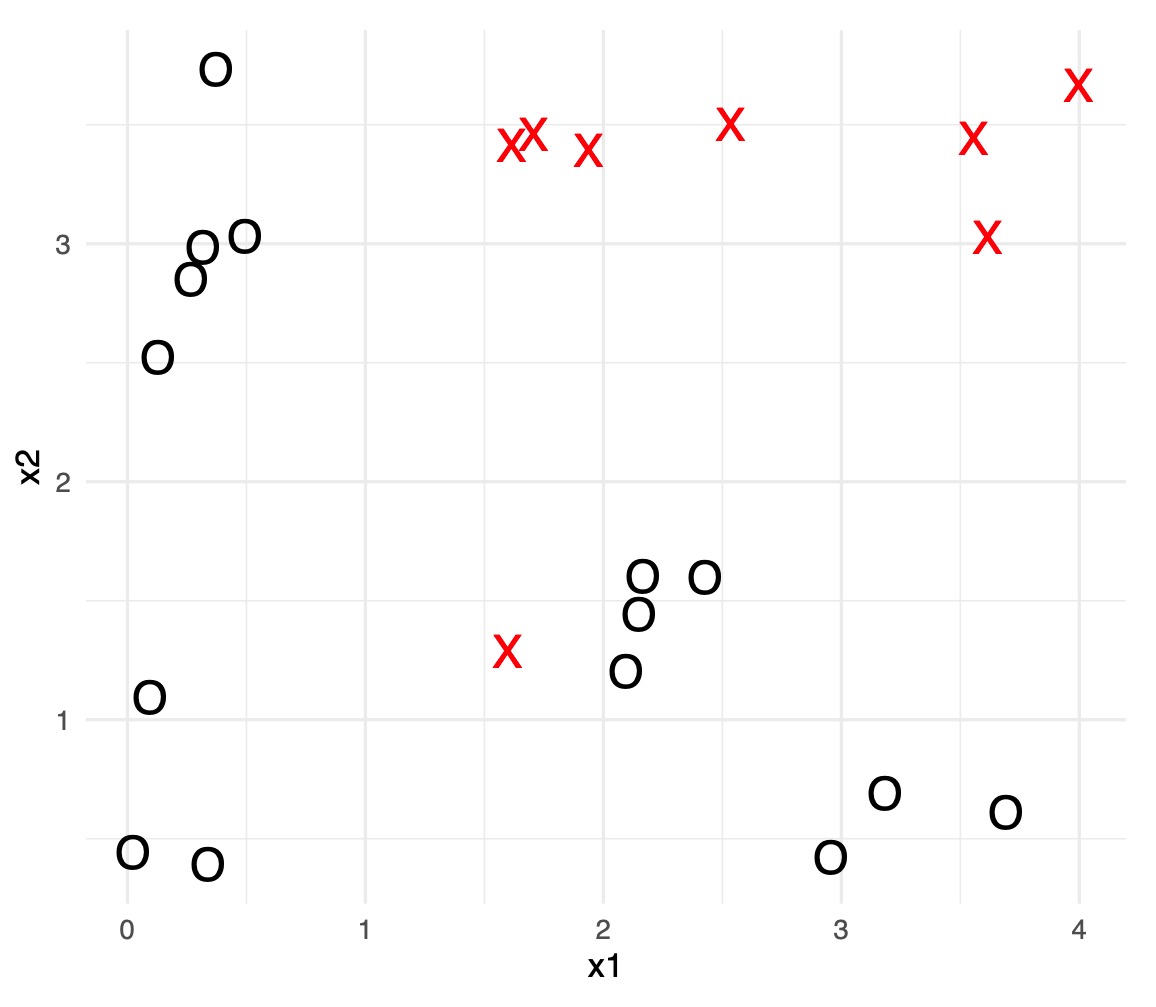
\includegraphics[width=16.06in]{data/p13}

In this task, you will simulate a decision tree algorithm by hand using
the toy data shown in the figure. Read Section 8.1 of ISLR\_v2. Use the
Gini index of Equation (8.6) as an impurity measure.

(You do not need to worry about overfitting here: the resulting
classification tree should have enough splits to fit the training data
without error. Don't worry if your results are not optimal or
super-accurate, as long as they are ``in the ballpark''.)

\hypertarget{problem-13-task-a}{%
\subsection{Problem 13 Task a}\label{problem-13-task-a}}

\begin{Shaded}
\begin{Highlighting}[]
\DecValTok{1}\SpecialCharTok{{-}}\NormalTok{((}\DecValTok{15}\SpecialCharTok{/}\DecValTok{23}\NormalTok{)}\SpecialCharTok{\^{}}\DecValTok{2}\SpecialCharTok{+}\NormalTok{(}\DecValTok{1{-}15}\SpecialCharTok{/}\DecValTok{23}\NormalTok{)}\SpecialCharTok{\^{}}\DecValTok{2}\NormalTok{)}
\DocumentationTok{\#\# [1] 0.4536862}
\DecValTok{1}\SpecialCharTok{{-}}\NormalTok{((}\DecValTok{8}\SpecialCharTok{/}\DecValTok{15}\NormalTok{)}\SpecialCharTok{\^{}}\DecValTok{2}\SpecialCharTok{+}\NormalTok{(}\DecValTok{1{-}8}\SpecialCharTok{/}\DecValTok{15}\NormalTok{)}\SpecialCharTok{\^{}}\DecValTok{2}\NormalTok{)}
\DocumentationTok{\#\# [1] 0.4977778}
\DecValTok{1}\SpecialCharTok{{-}}\NormalTok{((}\DecValTok{8}\SpecialCharTok{/}\DecValTok{12}\NormalTok{)}\SpecialCharTok{\^{}}\DecValTok{2}\SpecialCharTok{+}\NormalTok{(}\DecValTok{1{-}8}\SpecialCharTok{/}\DecValTok{12}\NormalTok{)}\SpecialCharTok{\^{}}\DecValTok{2}\NormalTok{)}
\DocumentationTok{\#\# [1] 0.4444444}
\DecValTok{1}\SpecialCharTok{{-}}\NormalTok{((}\DecValTok{4}\SpecialCharTok{/}\DecValTok{5}\NormalTok{)}\SpecialCharTok{\^{}}\DecValTok{2}\SpecialCharTok{+}\NormalTok{(}\DecValTok{1{-}4}\SpecialCharTok{/}\DecValTok{5}\NormalTok{)}\SpecialCharTok{\^{}}\DecValTok{2}\NormalTok{)}
\DocumentationTok{\#\# [1] 0.32}
\end{Highlighting}
\end{Shaded}

\begin{Shaded}
\begin{Highlighting}[]
\NormalTok{knitr}\SpecialCharTok{::}\FunctionTok{include\_graphics}\NormalTok{(}\FunctionTok{file.path}\NormalTok{(}\FunctionTok{here}\NormalTok{(), }\StringTok{"data"}\NormalTok{, }\StringTok{"tree.png"}\NormalTok{)) }
\end{Highlighting}
\end{Shaded}

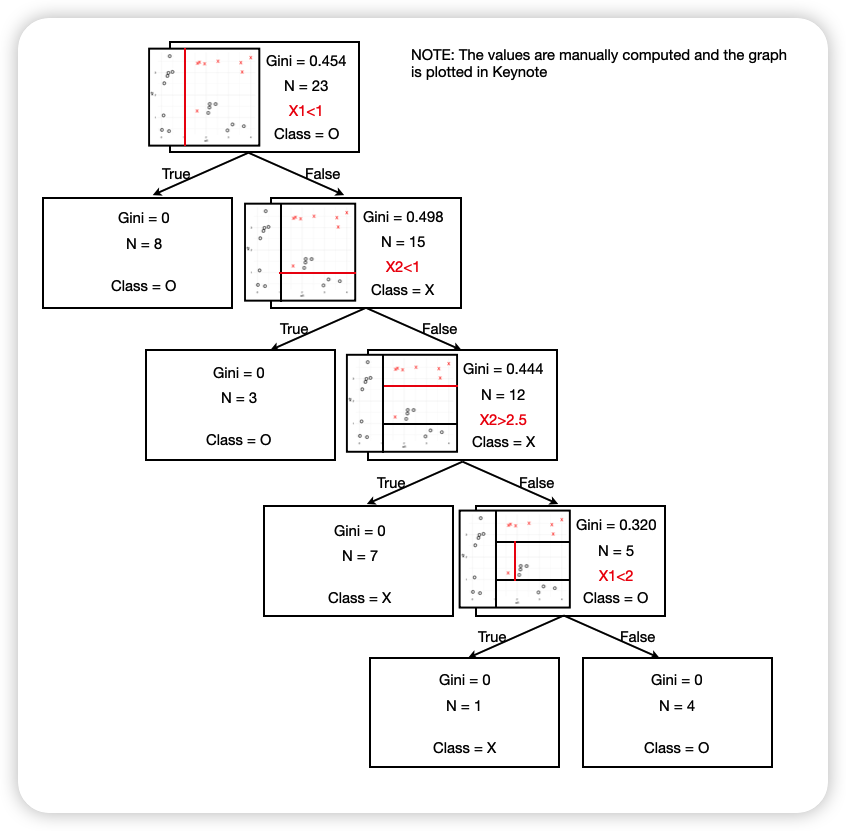
\includegraphics[width=11.75in]{data/tree}

\hypertarget{problem-14}{%
\section{Problem 14}\label{problem-14}}

Learning objectives: basics of the k-NN method.

In this task, you will apply the k-nearest neighbour (k-NN) classifier
by hand on a toy data set. You should be able to do this with pen and
paper. We will use the training dataset \(D = {(x_i, c_i)}_{i=1}^{14}\)
, shown below, where 𝑥 ∈ R are the co-variates and
\(c_i \in \{-1, +1\}\) are the classes.

\begin{Shaded}
\begin{Highlighting}[]
\NormalTok{p14.matrix }\OtherTok{\textless{}{-}} 
  \FunctionTok{matrix}\NormalTok{(}
    \FunctionTok{c}\NormalTok{(}\DecValTok{0}\NormalTok{,}\DecValTok{2}\NormalTok{,}\DecValTok{3}\NormalTok{,}\DecValTok{5}\NormalTok{,}\DecValTok{6}\NormalTok{,}\DecValTok{8}\NormalTok{,}\DecValTok{9}\NormalTok{,}\DecValTok{12}\NormalTok{,}\DecValTok{13}\NormalTok{,}\DecValTok{15}\NormalTok{,}\DecValTok{16}\NormalTok{,}\DecValTok{18}\NormalTok{,}\DecValTok{19}\NormalTok{,}\DecValTok{21}\NormalTok{, }\StringTok{"+1"}\NormalTok{,}\StringTok{"+1"}\NormalTok{,}\StringTok{"+1"}\NormalTok{,}\StringTok{"{-}1"}\NormalTok{,}\StringTok{"+1"}\NormalTok{,}\StringTok{"+1"}\NormalTok{,}\StringTok{"+1"}\NormalTok{,}\StringTok{"{-}1"}\NormalTok{,}\StringTok{"{-}1"}\NormalTok{,}\StringTok{"{-}1"}\NormalTok{,}\StringTok{"+1"}\NormalTok{,}\StringTok{"{-}1"}\NormalTok{,}\StringTok{"{-}1"}\NormalTok{,}\StringTok{"{-}1"}\NormalTok{),}
    \AttributeTok{nrow =} \DecValTok{2}\NormalTok{, }\AttributeTok{ncol =} \DecValTok{14}\NormalTok{, }\AttributeTok{byrow =}\NormalTok{  T}
\NormalTok{  )}
\FunctionTok{colnames}\NormalTok{(p14.matrix) }\OtherTok{\textless{}{-}} \DecValTok{1}\SpecialCharTok{:}\DecValTok{14}
\FunctionTok{rownames}\NormalTok{(p14.matrix) }\OtherTok{\textless{}{-}} \FunctionTok{c}\NormalTok{(}\StringTok{"xi"}\NormalTok{, }\StringTok{"ci"}\NormalTok{)}

\NormalTok{p14.matrix }\SpecialCharTok{|\textgreater{}}\NormalTok{ DT}\SpecialCharTok{::}\FunctionTok{datatable}\NormalTok{()}
\end{Highlighting}
\end{Shaded}

\includegraphics{E2_assignment_nocode_files/figure-latex/unnamed-chunk-33-1.pdf}

\hypertarget{problem-14-task-a}{%
\subsection{Problem 14 Task a}\label{problem-14-task-a}}

\hypertarget{question-11}{%
\subsubsection{Question}\label{question-11}}

Where are the classification boundaries for the 1-NN and 3-NN
classifiers? What are the respective classification errors on the
training dataset?

\hypertarget{my-answer-11}{%
\subsubsection{My answer}\label{my-answer-11}}

For 1-NN classifier, the classification boundaries are \textbf{4, 5.5,
10.5, 15.5 and 17}. The classification error is \textbf{0}.

For 3-NN classifier, the classification boundaries are \textbf{5.5,
10.5, 17}. The classification error is \textbf{0.143}.

\hypertarget{problem-14-task-b}{%
\subsection{Problem 14 Task b}\label{problem-14-task-b}}

\hypertarget{question-12}{%
\subsubsection{Question}\label{question-12}}

How does the choice of k in k-NN affect the classification boundary (not
in the above example but in general)? Give examples of the behaviour for
extreme choices (very small or large \(k\)).

\hypertarget{my-answer-12}{%
\subsubsection{My answer}\label{my-answer-12}}

The choice of K has a drastic effect on the KNN classifier obtained.
When K is extremely small, the decision boundary is overly flexible and
finds patterns in the data that don't correspond to the Bayes decision
boundary. This corresponds to a classifier that has low bias but very
high variance. As K grows, the method becomes less flexible and produces
a decision boundary that is close to linear. This corresponds to a
low-variance but high-bias classifier. For example, if we select
\(k = 1\), the classifier over-fits the data, leaving a training error
of 0 but high testing error; On the other hand, if we select a very
large k, say 100, the classifier will become less flexible with very big
variance, producing high testing error.

\hypertarget{problem-15}{%
\section{Problem 15}\label{problem-15}}

Topic: SVM

In this problem, you will study the support vector machine (SVM)
classifier on the toy data set shown below.

\begin{Shaded}
\begin{Highlighting}[]
\NormalTok{p15.matrix }\OtherTok{\textless{}{-}} 
  \FunctionTok{matrix}\NormalTok{(}
    \FunctionTok{c}\NormalTok{(}\SpecialCharTok{{-}}\FloatTok{1.5}\NormalTok{, }\DecValTok{0}\NormalTok{, }\DecValTok{1}\NormalTok{,}\DecValTok{0}\NormalTok{, }\FloatTok{0.9}\NormalTok{, }\DecValTok{1}\NormalTok{, }\FloatTok{0.2}\NormalTok{, }\SpecialCharTok{{-}}\FloatTok{1.8}\NormalTok{, }\DecValTok{1}\NormalTok{, }\DecValTok{2}\NormalTok{, }\DecValTok{0}\NormalTok{, }\DecValTok{1}\NormalTok{,}\DecValTok{4}\NormalTok{, }\DecValTok{1}\NormalTok{, }\SpecialCharTok{{-}}\DecValTok{1}\NormalTok{, }\DecValTok{4}\NormalTok{, }\SpecialCharTok{{-}}\DecValTok{1}\NormalTok{, }\SpecialCharTok{{-}}\DecValTok{1}\NormalTok{, }\DecValTok{6}\NormalTok{, }\SpecialCharTok{{-}}\FloatTok{0.5}\NormalTok{, }\SpecialCharTok{{-}}\DecValTok{1}\NormalTok{,  }\DecValTok{7}\NormalTok{, }\DecValTok{1}\NormalTok{, }\SpecialCharTok{{-}}\DecValTok{1}\NormalTok{),}
    \AttributeTok{nrow =} \DecValTok{8}\NormalTok{, }\AttributeTok{ncol =} \DecValTok{3}\NormalTok{, }\AttributeTok{byrow =}\NormalTok{ T}
\NormalTok{  )}

\FunctionTok{colnames}\NormalTok{(p15.matrix) }\OtherTok{\textless{}{-}} \FunctionTok{c}\NormalTok{(}\StringTok{"x1"}\NormalTok{, }\StringTok{"x2"}\NormalTok{, }\StringTok{"class"}\NormalTok{)}

\FunctionTok{rownames}\NormalTok{(p15.matrix) }\OtherTok{\textless{}{-}}\NormalTok{ LETTERS[}\DecValTok{1}\SpecialCharTok{:}\DecValTok{8}\NormalTok{]}
\end{Highlighting}
\end{Shaded}

Find a separating hyperplane with the largest margin on the data set
above. write down the equation for this hyperplane and report the margin
size.

Which of the points(A-H) are support vectors?

Hint: You can answer without mathematical proofs. You can do it simply
by geometric intuition.

\begin{Shaded}
\begin{Highlighting}[]
\NormalTok{knitr}\SpecialCharTok{::}\FunctionTok{include\_graphics}\NormalTok{(}\FunctionTok{file.path}\NormalTok{(}\FunctionTok{here}\NormalTok{(), }\StringTok{"data"}\NormalTok{, }\StringTok{"p15.png"}\NormalTok{)) }
\end{Highlighting}
\end{Shaded}

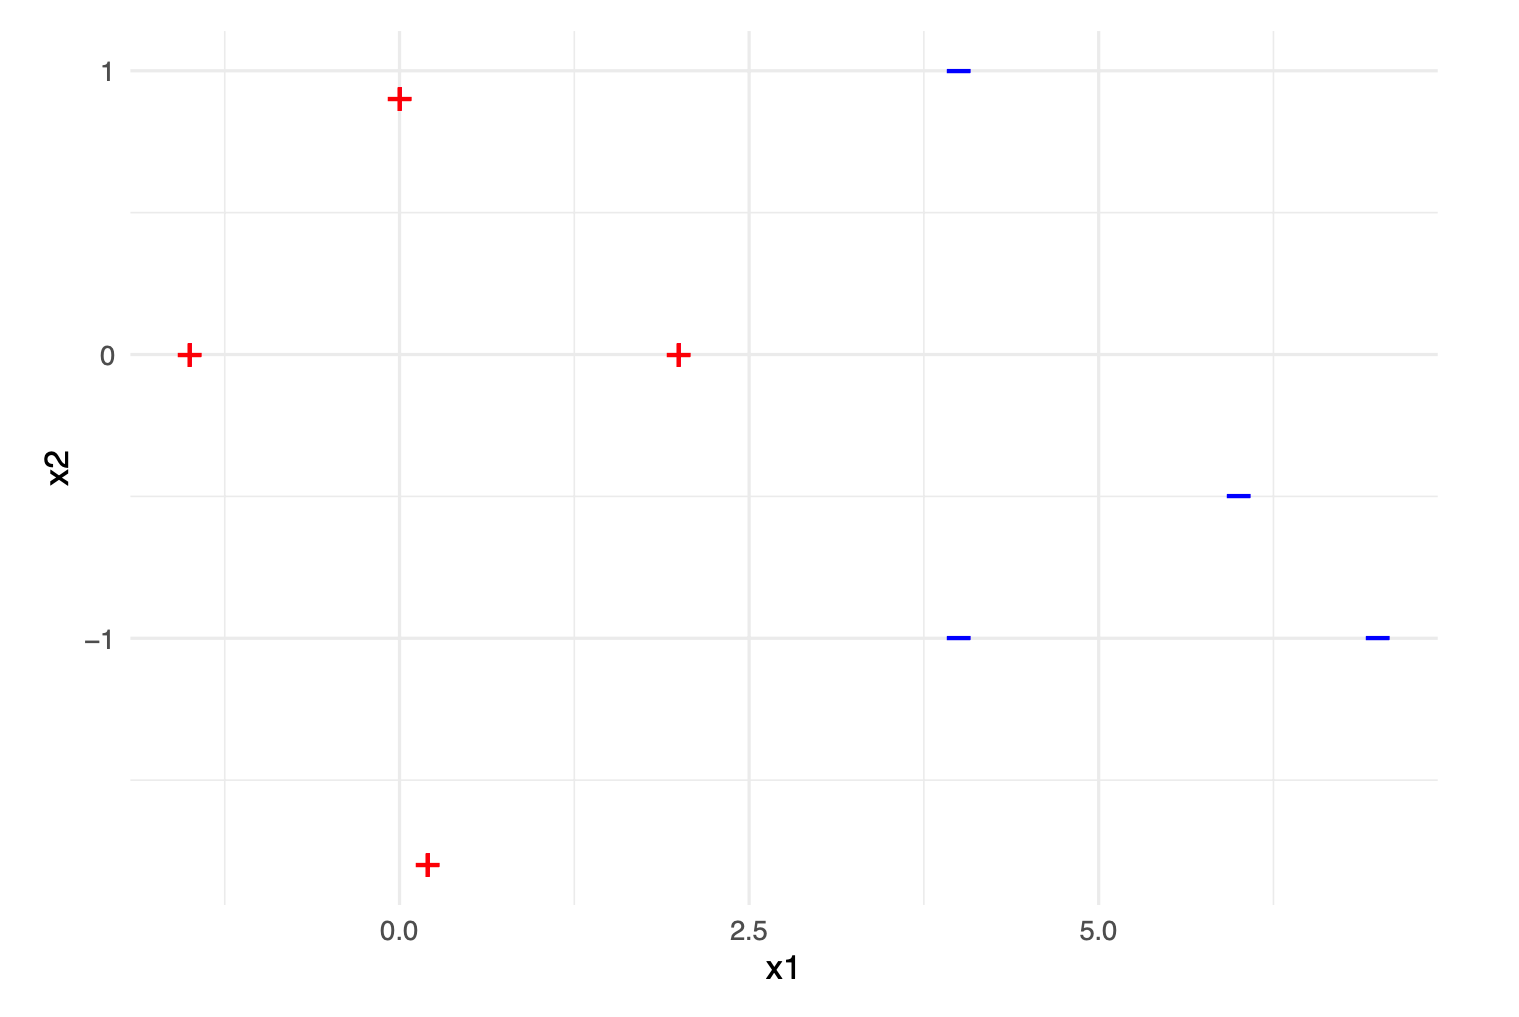
\includegraphics[width=21.1in]{data/p15}

My intuition is points D, E and F are support vectors. The points are
plotted as below, with hyperlane plotted as a thick line and points on
dashed lines are support vectors.

\begin{Shaded}
\begin{Highlighting}[]
\CommentTok{\# Given dataset matrix}
\NormalTok{p15.matrix }\OtherTok{\textless{}{-}} 
  \FunctionTok{matrix}\NormalTok{(}
    \FunctionTok{c}\NormalTok{(}\SpecialCharTok{{-}}\FloatTok{1.5}\NormalTok{, }\DecValTok{0}\NormalTok{, }\DecValTok{1}\NormalTok{, }\DecValTok{0}\NormalTok{, }\FloatTok{0.9}\NormalTok{, }\DecValTok{1}\NormalTok{, }\FloatTok{0.2}\NormalTok{, }\SpecialCharTok{{-}}\FloatTok{1.8}\NormalTok{, }\DecValTok{1}\NormalTok{, }\DecValTok{2}\NormalTok{, }\DecValTok{0}\NormalTok{, }\DecValTok{1}\NormalTok{, }\DecValTok{4}\NormalTok{, }\DecValTok{1}\NormalTok{, }\SpecialCharTok{{-}}\DecValTok{1}\NormalTok{, }\DecValTok{4}\NormalTok{, }\SpecialCharTok{{-}}\DecValTok{1}\NormalTok{, }\SpecialCharTok{{-}}\DecValTok{1}\NormalTok{, }\DecValTok{6}\NormalTok{, }\SpecialCharTok{{-}}\FloatTok{0.5}\NormalTok{, }\SpecialCharTok{{-}}\DecValTok{1}\NormalTok{, }\DecValTok{7}\NormalTok{, }\DecValTok{1}\NormalTok{, }\SpecialCharTok{{-}}\DecValTok{1}\NormalTok{),}
    \AttributeTok{nrow =} \DecValTok{8}\NormalTok{, }\AttributeTok{ncol =} \DecValTok{3}\NormalTok{, }\AttributeTok{byrow =}\NormalTok{ T}
\NormalTok{  )}

\CommentTok{\# Convert matrix to data frame for plotting}
\NormalTok{p15.df }\OtherTok{\textless{}{-}} \FunctionTok{as.data.frame}\NormalTok{(p15.matrix)}
\FunctionTok{colnames}\NormalTok{(p15.df) }\OtherTok{\textless{}{-}} \FunctionTok{c}\NormalTok{(}\StringTok{"x1"}\NormalTok{, }\StringTok{"x2"}\NormalTok{, }\StringTok{"class"}\NormalTok{)}
\FunctionTok{plot}\NormalTok{(p15.df}\SpecialCharTok{$}\NormalTok{x1, p15.df}\SpecialCharTok{$}\NormalTok{x2, }\AttributeTok{col=}\FunctionTok{factor}\NormalTok{(p15.df}\SpecialCharTok{$}\NormalTok{class), }\AttributeTok{pch=}\DecValTok{19}\NormalTok{, }\AttributeTok{xlab=}\StringTok{"x1"}\NormalTok{, }\AttributeTok{ylab=}\StringTok{"x2"}\NormalTok{)}

\FunctionTok{abline}\NormalTok{(}\AttributeTok{v=}\DecValTok{3}\NormalTok{, }\AttributeTok{lwd =} \DecValTok{3}\NormalTok{) }

\FunctionTok{abline}\NormalTok{(}\AttributeTok{v=}\DecValTok{2}\NormalTok{, }\AttributeTok{lty =} \DecValTok{2}\NormalTok{) }
\FunctionTok{abline}\NormalTok{(}\AttributeTok{v=}\DecValTok{4}\NormalTok{, }\AttributeTok{lty =} \DecValTok{2}\NormalTok{) }
\end{Highlighting}
\end{Shaded}

\includegraphics{E2_assignment_nocode_files/figure-latex/unnamed-chunk-36-1.pdf}

The Hyperplane Equations for points D, E and F are

\begin{itemize}
\item
  D: \(a \times 2.0 + b \times 0 + c = 0\)
\item
  E: \(a \times 4.0 + b \times 1 + c = 0\)
\item
  F: \(a \times 4.0 + b \times -1 + c = 0\)
\end{itemize}

\hypertarget{problem-16}{%
\section{Problem 16}\label{problem-16}}

\hypertarget{problem-16-task-a}{%
\subsection{Problem 16 Task a}\label{problem-16-task-a}}

\hypertarget{question-13}{%
\subsubsection{Question}\label{question-13}}

Write a learning diary of the topics of lectures 5-8 and this exercise
set.

Instructions

Guiding questions: What did I learn? What did I not understand? Was
there something relevant to other studies or (future) work? Your reply
should be 1-3 paragraphs of text. You can also give feedback on the
course.

During these sessions, I learnt the logic behind a number of
classifiers, including logistic regression, LDA, naive Bayesian, SVM,
decision trees, bagging, random forests and ensemble methods. I followed
the math behind some of these techniques. I also reviewed a number of
distance metrics.

I didn't manage to follow some of the mathematical proofs, especially
support vector machine. Some of the distance metrics mentioned in the
class sounds very new to me. I am still trying to get my head around
them, especially which metrics fits which scenario.

In the sessions I found some math blind spots (such as optimization) and
I will make them up by joining more basic level courses, after this
course.

\hypertarget{problem-16-task-b}{%
\subsection{Problem 16 Task b}\label{problem-16-task-b}}

\hypertarget{question-14}{%
\subsubsection{Question}\label{question-14}}

Give an estimate of the hours used in solving the problems in this
exercise set.

\hypertarget{my-answer-13}{%
\subsubsection{My answer}\label{my-answer-13}}

12 hours.

\end{document}
